\begin{justifying}
  \noindent 
  Hasta ahora no hemos abordado el cambio. Pero, si creemos en la ciencia, debemos defender el postulado ontológico de que todo 
  está en constante cambio. De hecho, las ciencias describen, explican, predicen, 
  controlan o provocan cambios de diversos tipos, como el movimiento, la acreción, 
  la división y la evolución. Por lo tanto, la ontología debería analizar y sistema tizar estos diversos tipos de cambio.
  Mientras algunos metafísicos se han dedicado a elogiar el cambio, otros lo han negado y ninguno lo ha descrito correctamente. Nos esforzaremos por construir un concepto de cambio lo suficientemente amplio y, por lo tanto, lo suficientemente pobre como para abarcar todos los conceptos de cambio, en particular los que se dan en las ciencias, y esbozar teorías generales del cambio de algunos tipos típicos. Estos son los objetivos del presente capítulo, dedicado al cambio en general. El tema del cambio cualitativo se abordará en el volumen complementario, \textit{Un Mundo de Sistemas}.
  Un cambio es un evento o un proceso, ya sea cuantitativo, cualitativo o ambos. Sea cual sea su naturaleza, un cambio es una modificación en o de alguna cosa o cosas: más precisamente, consiste en una variación del estado de una entidad. Dicho de forma negativa, no existe cambio separado de las cosas; ni, de hecho, existen cosas inmutables, aunque algunas cambien lentamente o solo en ciertos aspectos limitados. El mundo, entonces, consiste en cosas que no permanecen en el mismo estado para siempre. Esta hipótesis metafísica es una extrapolación tanto de la experiencia ordinaria como del conocimiento científico. La hipótesis contraria, que nada cambia, es una extravagancia filosófica poco digna de la consideración de una persona cuerda.

  \newpage

	\noindent Conocimiento de la naturaleza de la cosa en cuestión: por lo tanto,
	es idealmente adecuado para la ontología o la teoría general de las cosas.
	Comencemos entonces recordando brevemente las nociones de estado y espacio de estados,
	para adentrarnos inmediatamente al fondo del asunto.

	\section{\centering \large CAMBIABILIDAD}
	\subsection{Preliminares}
	\noindent Todo se encuentra en un estado u otro en relación con un marco de referencia determinado.
	Y cada estado (relativo) de una cosa viene determinado de forma única por las
	propiedades de esta última (en relación con algún marco). Por lo tanto, el estado de una cosa
	con n propiedades, cada una representada por una función (de estado), es una n-tupla de
	valores de las funciones que representan esas propiedades. Los diferentes estados
	corresponden a (están representados por) diferentes n-tuplas. Un cambio en la
	representación de las propiedades, o en la elección del marco de referencia, da lugar a
	una representación diferente de los estados. Esto demuestra que nuestro conocimiento de
	un estado depende en parte de nosotros mismos y del estado de la técnica, pero no
	de que el estado en sí mismo sea un artefacto del observador. En resumen, los estados
	son relativos.

	Supongamos, para mayor precisión, que un objeto x, como el obturador de una cámara o un interruptor 
    eléctrico, tiene una única propiedad general dicotómica: que está abierto (1) o cerrado (0). 
    Los posibles estados de x son entonces 0 y 1. En otras palabras, el espacio de estados de x es S(x)={O, I}.
    En realidad, esto es una simplificación excesiva: 0 y 1 son solo los estados de interés para algunos propósitos 
    específicos. Cualquier objeto real tiene un gran número n de propiedades Pi', cada una representable por una función Fj, donde 1 ~ i ~ n.
    Los posibles grados o intensidades de la propiedad Pi se representan como tantos valores de la función Fj. 
    Por lo tanto, el espacio de estados concebible del objeto será el producto vectorial de las imágenes de estas funciones. 
    Y el espacio de estados nomológico será un subconjunto del espacio anterior, resultante de las leyes que involucran a Pi: 
    véase la Figura 5.1. Todo esto es válido, por supuesto, para una representación dada de propiedades, y por tanto de estados.


	\begin{center}
		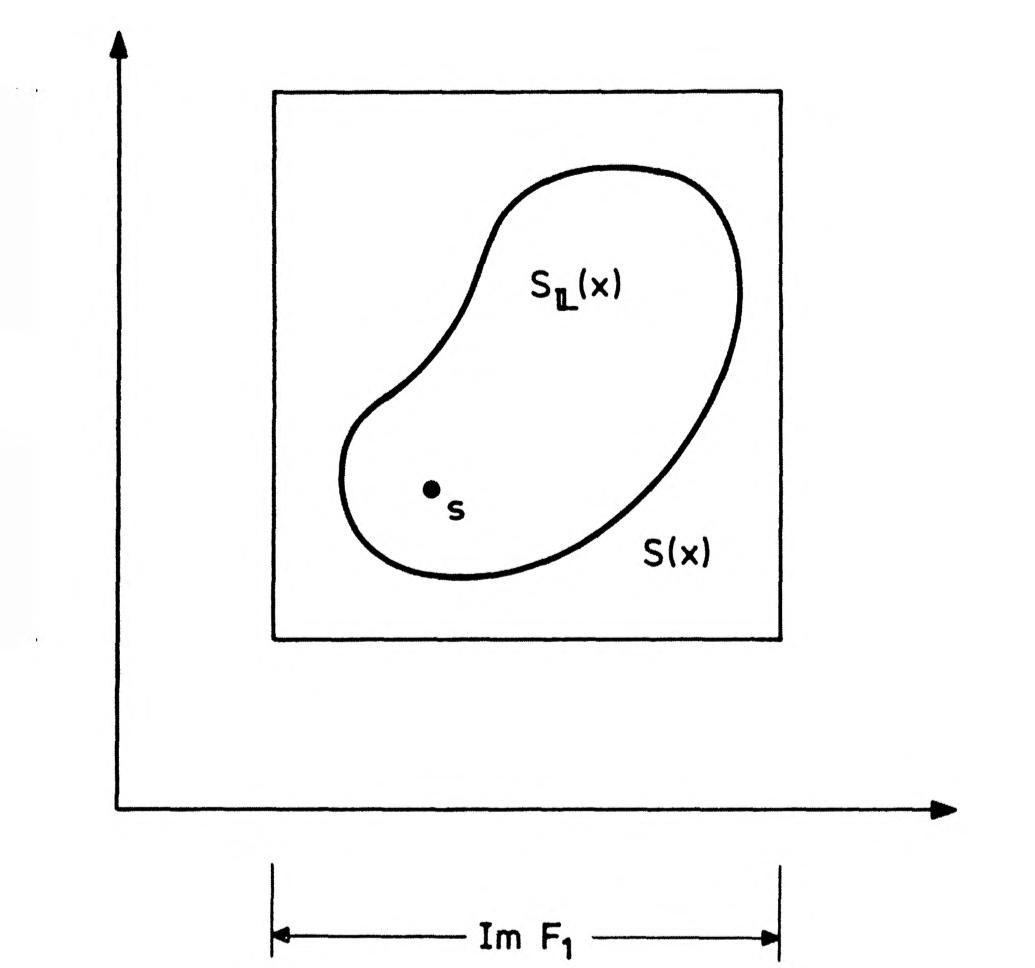
\includegraphics[width=0.6\textwidth]{img/Figura5-1.png}
		\\ \scriptsize Fig. 5.l. El espacio de estados concebible $S(x)$ y el espacio de estados legítimo $S_\mathrm{L}(x)$ de una cosa $x$
		con dos propiedades representadas por las funciones $F_\mathrm{1}$ y $F_\mathrm{2}$.
		\textit{'$F$'} se lee \textit{'la imagen $F$'} es el conjunto de valores, o rango, de $F$.
	\end{center}


	\noindent la curva con la ayuda de un parámetro, cuya interpretación estándar es el tiempo.
	Pero una de las ventajas de la representación del cambio en el espacio de estados
	es que no requiere el uso explícito del concepto de tiempo.

	Para aclarar las ideas, consideremos el espacio de estados del conjunto genético de una población
	de organismos. Ese conjunto está incluido en el espacio cartesiano cuyos ejes son
	las frecuencias genéticas del conjunto. Cada punto de este espacio representa un estado posible del conjunto genético. El punto representativo, el que representa el estado real del sistema, permanecerá fijo solo si los organismos no sufren mutaciones, lo que nunca ocurre, ni siquiera si el entorno de la población es muy estable, como una laguna tropical.
	De lo contrario, el punto representativo se mueve (en el espacio de estados, no en el espacio ordinario) describiendo una trayectoria. Esta curva, que en el caso de la evolución biológica no tiene bucles, representa la historia genética del conjunto genético.
	De lo contrario, el punto representativo se mueve (en el espacio de estados, no en el espacio ordinario)
	describiendo una trayectoria. Esta curva, que en el caso de la
	evolución biológica no tiene bucles , representa la historia genética del
	pool genético, o la evolución de la población correspondiente a nivel genético.
	Cualquier segmento de la historia total puede denominarse evento o
	proceso que involucra al pool genético. (Véase la figura 5.2).

	\begin{center}
		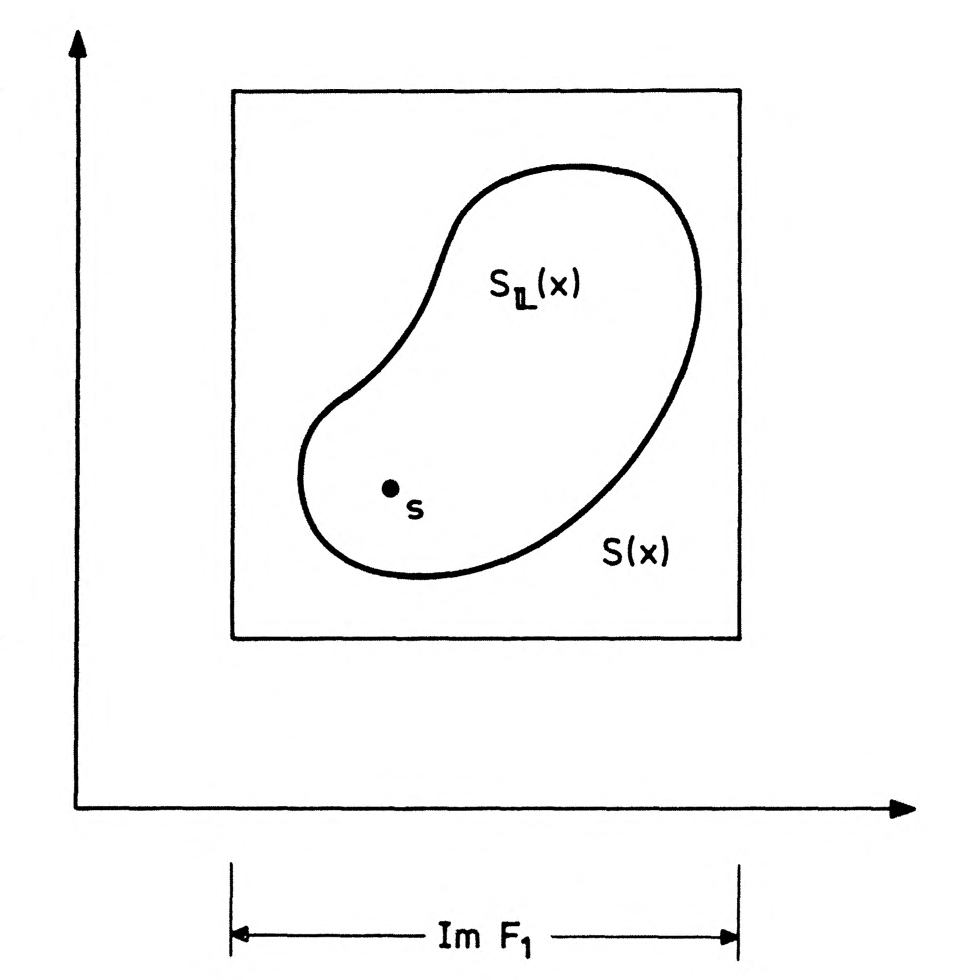
\includegraphics[width=0.6\textwidth]{img/Figura5-2.png}
		\\ \scriptsize Fig. 5.2. El cambio en las frecuencias genéticas en un acervo genético,
		en respuesta a la acción conjunta de la mutación y la selección.
		Los extremos de la curva representan el origen y la extinción de la población dada.
	\end{center}
    Demasiado para un trasfondo intuitivo.

    \subsection{Capacidad de cambio}
    \noindent Antes de abordar el cambio real, conviene aclarar la noción intuitiva
    de mutabilidad o variabilidad:

    \bigskip

    \noindent DEFINICIÓN 5.1: Sea $x$ una cosa. Entonces
    \begin{enumerate}[label=(\roman*), itemsep=0pt, parsep=0pt]
        \item $x$ es inmutable si y solo si $S_\mathrm{L}(x)$ es un singleton para todas las elecciones de función de estado para $x$.
        \item $x$ es cambiante (o mutable) si y solo si $S_\mathrm{L}(x)$ tiene al menos dos miembros distintos
            para todas las elecciones de función de estado para $x$.
    \end{enumerate}

    \bigskip

    \noindent POSTULADO 5.1 Toda cosa (concreta) tiene al menos dos estados distintos y 
    el espacio de estados de cualquier construcción está vacío. Es decir:
    \begin{enumerate}[label=(\roman*), itemsep=0pt, parsep=0pt]
        \item si $x$ es una cosa, entonces, para todas las elecciones de la función de estado para $x$, $|S_\mathrm{L}(x)| \geq 2$.
        \item si y es una construcción, entonces no hay funciones de estado para $y$, $o$, equivalentemente, $S_\mathrm{L}(y) = \varnothing$.
    \end{enumerate}

    Una consecuencia inmediata del Postulado 5.1 y la Definición 5.1 es

    \bigskip

    \noindent COROLARIO 5.1 Todas las cosas (concretas) son cambiantes, y las construcciones
    no son ni inmutables ni cambiantes.

    Observación 1. No estamos afirmando (todavía) que todo esté realmente
    sufriendo algún tipo de cambio, sino solo que puede cambiar. Observación
    2. La segunda parte del Corolario 5.1 afirma que las categorías de cambio
    e inmutabilidad no se aplican a los constructos. Los constructos no son ni
    objetos eternos (Platón) ni cambiantes (Hegel). Lo que cambia
    de una persona a otra son los procesos cerebrales que se producen cuando se piensan los constructos. \\
	Nuestro siguiente concepto es el del cambio global, independientemente del orden en que se produzca:

    \bigskip

    \noindent DEFINICIÓN 5.2 Sea $S_\mathrm{L}(x)$ un espacio de estados legítimo de una cosa $x$, y sean $S_\mathrm{i}(x)$, 
    $S_\mathrm{j}(x) \subset S_\mathrm{L}(x)$ dos colecciones de estados de $x$ [por ejemplo, dos regiones de
    $S_\mathrm{L}(x)$]. Entonces, el cambio global de $x$ entre $S_\mathrm{i}(x)$ y$S_\mathrm{i}(x)$ es igual a la
    diferencia simétrica entre los subconjuntos dados:

	\medskip

	$X_\mathrm{ij}(x) \:= \:S_\mathrm{i}(x) \:\triangle \: S_\mathrm{j}(x)$.

	\medskip

	Un cambio general puede ser leve o grande, superficial o profundo. Si
	hay cambios considerables en las propiedades individuales de una cosa, pero la
	cosa no adquiere ni pierde ninguna propiedad general, podemos decir que
	sufre un gran cambio. Si, por el contrario, una cosa gana o pierde
	propiedades generales, entonces se puede decir que sufre un cambio profundo.
	Mientras que en el primer caso los ejes del espacio de estados permanecen fijos, en el
	segundo se añaden o se eliminan algunos. Obtenemos una descripción fluida de
	este tipo de cambio si construimos el espacio de estados con todos los ejes necesarios
	y utilizamos en cada momento solo aquellas partes del espacio total que
	se refieren a las propiedades que realmente posee la cosa en ese momento. En la
	figura 5.3 representamos la evolución de una cosa imaginaria que sufre un
	cambio profundo. La primera parte del proceso se describe mediante una curva en el
	plano horizontal $lm \: F_\mathrm{1} \times lm \: F_\mathrm{2}$; la segunda parte se describe mediante una curva
	en el plano vertical. El cambio cualitativo se produce en la
	unión de las dos curvas. Toda la curva es continua, aunque
	su tangente tenga una discontinuidad.

	\bigskip

	\begin{center}
		\title{\normalsize CAPITULO 5}
	\end{center}

	\smallskip

	\begin{center}
		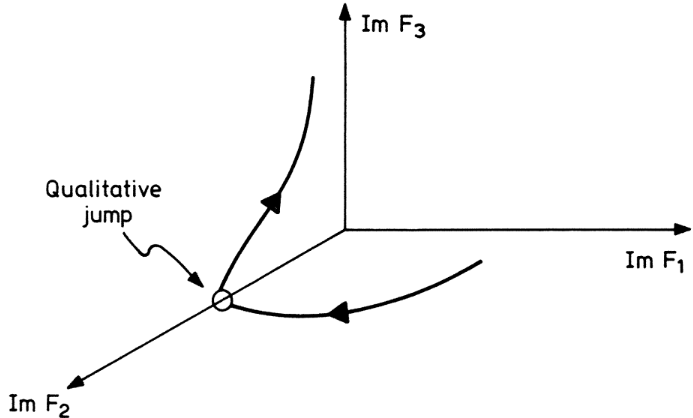
\includegraphics[width=0.7\textwidth]{img/Figura5-3.png}
		\\ \scriptsize Fig. 5.3. Cada arco de la curva describe un cambio cuantitativo. 
		Un salto cualitativo ocurre en la unión de los dos arcos.
	\end{center}

	\bigskip

	En otras palabras, adoptamos

	\bigskip

	\noindent DEFINICIÓN 5.3 Sea $\mathbb{F}$ una función de estado que abarca todo el espacio de estados
	$S_\mathrm{L}(x)$ para una cosa $x$. La cosa sufre un \textit{cambio cualitativo} si y solo si
	$S_\mathrm{L}(x)$ es igual a la unión de al menos dos subespacios, cada uno de los cuales está
	abarcado por una proyección diferente de $\mathbb{F}$. De lo contrario [es decir, si ninguno de los
	componentes puede ignorarse durante ninguna parte del proceso], la cosa
	solo sufre un \textit{cambio cuantitativo}.

	Una consecuencia inmediata de esta definición es

	\bigskip

	COROLARIO 5.2 Todo cambio cualitativo va acompañado de un cambio cuantitativo.
	[Es decir, para cualquier cosa $x$, si $x$ cambia cualitativamente, entonces $x$ cambia cuantitativamente].

	Lo contrario no se cumple, lo cual es mejor, ya que es falso.
	Tenga en cuenta que lo anterior no es una hipótesis ontológica independiente, sino un
	mero corolario de una convención. El problema es que esta última se ha
	formulado de manera que se obtenga esa consecuencia.

	Hasta aquí la distinción entre cualitativo y cuantitativo. El presente
	capítulo se dedicará al cambio en general; el cambio cualitativo se tratará
	en el siguiente volumen de este tratado.

	\newpage

	\begin{center}
		\title{\normalsize CAMBIO}
	\end{center}

	\section{\centering Evento}

	\subsection{\normalsize \textit{La representación ordenada por pares de los eventos}}
	\noindent Cualquier cambio puede considerarse como una transformación en algo diferente
	o como una transición a un estado diferente. En el primer caso, el cambio de
	interés puede interpretarse como el par ordenado $\langle x, x' \rangle$, donde $x$ y $x'$
	son las cosas inicial y final, respectivamente. Sin embargo, dado que los nombres o
	términos singulares como $`x`$ y $`x'`$ no son descriptivos, esta representación
	del cambio no es esclarecedora. Además, obliga a una multiplicación innecesaria
	del número de cosas. Por esta razón, no se utiliza en ciencia
	y no la emplearemos en ontología.

	Se transmite mucha más información si el nombre `$x$' se sustituye por la
	frase `la cosa $x$ está en el estado $s$', donde $s$ es un punto (o un conjunto de puntos) en un
	espacio de estados $S_\mathrm{L}(x)$ para $x$. Entonces podemos interpretar un cambio de $x$ como una transición
	del estado $s$ a algún otro estado $s' \in S_\mathrm{L}(x)$. En otras palabras, adoptamos lo que
	podría denominarse el \textit{principio de invariancia nominal}, o permanencia de los
	nombres a través del cambio, y describimos los cambios como cambios de estado. El
	principio, una regla de designación, puede enunciarse de la siguiente manera:

	\bigskip

	\noindent PRINCIPIO 5.1 Una cosa, si se le da un nombre, mantendrá ese nombre a lo largo de su
	historia, siempre y cuando esta no incluya cambios en su naturaleza,
	cambios que requieran cambios de nombre.

	Para que este principio funcione, debemos incluir en el espacio de estados de
	una cosa todos los estados posibles de esta, desde el principio hasta el final. Esto
	nos permite designar a una persona determinada a los 50 años con el mismo nombre que a los
	5 años, aunque entre medias la persona haya renovado cada uno de los
	átomos de su cuerpo. En resumen, no hay cosas autoidenticas, sino solo
	nombres constantes que nos ayudan a seguir los cambios que experimentan
	las cosas.

	En cuanto al principio de representación, una suposición semántica, se puede formular así:
	El principio de representación es la idea de que la representación es una forma de conocimiento.

	\newpage

	\begin{center}
		\title{\normalsize CAPITULO 5}
	\end{center}

	\noindent PRINCIPIO 5.2 Sea $S(x)$ un espacio de estados para una cosa $x$, y sean $s, s' \in S(x)$
	dos estados de $x$. Entonces, el cambio neto en $x$ del estado $s$ al estado $s'$ es
	representable por el par ordenado de estos estados, es decir, por $\langle s, s' \rangle \in
	S(x) \times S(x)$.

	En el caso más simple no trivial (aunque imaginario), $S(x) = \{a, b\}$, y existe
	una única función $g: S(x) \to S(x)$ tal que $g(a)=b$ y $g(b)=a$, para representar los dos posibles cambios no triviales de la cosa, a saber $(a, b)$
	y $(b, a)$. La permanencia se representa mediante la función $es: S(x) \to S(x)$
	tal que $es(a) = a$ y $es(b) = b$, es decir, la función identidad en $S$.

	Los principios anteriores son la clave de la teoría del cambio que se desarrollará en
	la secuela. Primero abordamos el caso más simple del espacio de estados finito,
	y después el caso general.

	\bigskip

	\subsection{\textit{El espacio para eventos}}

	\noindent Sea $S(x)$ un espacio de estados para una cosa $x$. Cualquier par de puntos en este conjunto
	representará de manera inequívoca, aunque quizás no exhaustiva, un evento
	o cambio concebible en $x$. (Concebible en lugar de realmente posible
	porque $(a)$ $S(x)$ en sí mismo es la colección de estados concebibles de $x$, y $(b)$
	incluso si se considera que $S(x)$ es un espacio de estados legítimo, no todas las transiciones
	desde o hacia un estado dado pueden ser realmente posibles. Basta con pensar en el espacio de estados
	$S(x) = {vivo, muerto}$.)

	En esta sección investigaremos la pertenencia y la estructura precisas
	del espacio $E(x)$ de eventos concebibles. Comenzamos examinando
	el caso simple de una cosa con tres estados, como un interruptor eléctrico con tres
	estados: abierto, cerrado y transitorio. Llamando $a$, $b$ y $c$ a los estados, tenemos
	$S(x) = {a, b, c}$. Ahora formamos los pares ordenados

	\begin{itemize}[itemsep=0pt, parsep=0pt]
		\item [ ] $\langle a, a \rangle $ la cosa $x$ permanece en el estado $a$ (el evento de identidad en $a$)
		\item [ ] $\langle a, b \rangle$ la cosa $x$ pasa del estado $a$ al estado $b$, etc.
	\end{itemize}

	Cada uno de estos pares representa un cambio concebible en x, es decir, un
	evento concebible que involucra a $x$. Supongamos además, por conveniencia,
	que en este caso particular todos esos eventos pueden ocurrir, es decir, son
	legítimos. En otras palabras, establezcamos $E_\mathrm{L}(x) \: = \: E(x) \: = \: S(x) \: \times \: S(x)$. Así, tenemos 9
	eventos elementales o no compuestos en $E(x)$:
	
	\begin{center}
		\begin{tabular}{l c r}
			$e_\mathrm{1} = \langle a, a \rangle =u_\mathrm{a'}$ & $e_\mathrm{4} = \langle a, b \rangle,$ & $e_\mathrm{7} = \langle b, a \rangle$ \\
			$e_\mathrm{2} = \langle b, b \rangle = u_\mathrm{b'}$ & $e_\mathrm{5} = \langle b, c \rangle,$ & $e_\mathrm{8} = \langle c, b \rangle$ \\
			$e_\mathrm{3} = \langle c, c \rangle = u_\mathrm{c'}$ & $e_\mathrm{6} = \langle a, c \rangle,$ & $e_\mathrm{9} = \langle c, a \rangle.$
		\end{tabular}
	\end{center}

	\noindent Es decir, $E(x) = ^2(X) = \{u_a, u_b, u_c, e_4, e_5, e_6, e_7, e_8, e_9\}$. Los tres primeros
	elementos de este conjunto son no sucesos o cambios nulos. Por lo tanto, $U_\mathrm{a}$ es el
	no suceso que consiste en que la cosa permanece en el estado $a$. Todos los demás son
	sucesos propiamente dichos. En la figura 5.4 se muestra una representación gráfica estándar de este espacio.

	\begin{center}
		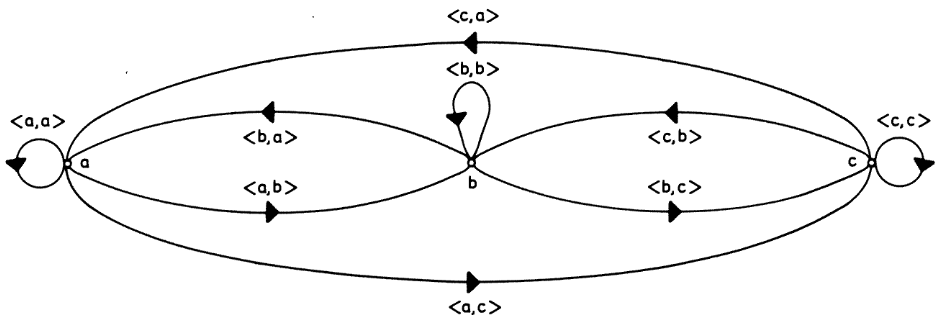
\includegraphics[width=1\textwidth]{img/Figura5-4.png}
		\\ \scriptsize Fig. 5.4. El gráfico de transición o de Moore para un elemento de tres estados.
	\end{center}

	Suponemos a continuación que la composición de ciertos eventos es posible,
	mientras que la de otros no lo es. Por ejemplo, el evento $e_4 = \langle a, b \rangle$ puede ir seguido
	del evento $e_5 = \langle b, c \rangle$, y el evento complejo puede considerarse como una
	descomposición del evento $e_6 = \langle a, c \rangle$. Para simbolizar la composición de
	eventos, utilizamos el asterisco * y escribimos: $e_4 * e_5 = e_6$ o, explícitamente,
	$\langle a, b \rangle * \langle b, c \rangle = \langle a, c \rangle$. (Es decir, los estados
	intermedios no aparecen en el cambio neto: se absorben). Por otro lado, el evento complejo
	$\langle b, c \rangle * \langle a, b \rangle$, que es el inverso del anterior, no se produce,
	por lo que queda sin definir. En otras palabras, para representar la combinación de
	eventos, introducimos una operación binaria (parcial) * en: $E(x)$. Si $e$ y $f$ están
	en $E(x)$, entonces $e * f = g$ es otro evento en $E(x)$ que consiste en que el evento $e$
	es seguido por el evento $f$, con la salvedad de que, en ciertos casos, la
	composición no está definida.
	
	Las posibles combinaciones binarias de eventos que ocurren en una cosa de tres estados
	se muestran en la siguiente tabla. Cada entrada de esta tabla de multiplicación
	muestra el cambio neto, no el proceso de cambio. Pero, por supuesto, el\

	\begin{center}
			\setlength{\tabcolsep}{3pt}
			\footnotesize \begin{tabular}{c|ccccccccc}
				* & $\langle a,a \rangle$ & $\langle a,b \rangle$ & $\langle a,c \rangle$ & $\langle b,a \rangle$ & $\langle b,b \rangle$ & $\langle b,c \rangle$ & $\langle c,a \rangle$ & $\langle c,b \rangle$ & $\langle c,c \rangle$ \\
				\hline
				$\langle a,a \rangle$ & $\langle a,a \rangle$ & $\langle a,b \rangle$ & $\langle a,c \rangle$ & & & & & & \\
				$\langle a,b \rangle$ &  &  &  & $\langle a,a \rangle$ & $\langle a,b \rangle$ & $\langle a,c \rangle$ & & & \\
				$\langle a,c \rangle$ &  &  &  &  &  &  & $\langle a,a \rangle$ & $\langle a,b \rangle$ & $\langle a,c \rangle$ \\
				$\langle b,a \rangle$ & $\langle b,a \rangle$ & $\langle b,b \rangle$ & $\langle b,c \rangle$ & & & & & & \\
				$\langle b,b \rangle$ &  & & & $\langle b,a \rangle$ & $\langle b,b \rangle$ & $\langle b,c \rangle$ & & & \\
				$\langle b,c \rangle$ &  & & & & & & $\langle b,a \rangle$ & $\langle b,b \rangle$ & $\langle b,c \rangle$ \\
				$\langle c,a \rangle$ & $\langle c,a \rangle$ & $\langle c,b \rangle$ & $\langle c,c \rangle$ & & & & & & \\
				$\langle c,b \rangle$ &  & & & $\langle c,a \rangle$ & $\langle c,b \rangle$ & $\langle c,c \rangle$ & & & \\
				$\langle c,c \rangle$ &  &  & & & & & $\langle c,a \rangle$ & $\langle c,b \rangle$ & $\langle c,c \rangle$ \\
			\end{tabular}
	\end{center}

	\noindent La tabla nos permite analizar ciertos eventos como procesos, es decir, secuencias de eventos elementales.
	De esta tabla se desprenden claramente una serie de regularidades. Suponemos
	que son válidas para todos los espacios de eventos y las resumimos en

	\bigskip

	\noindent DEFINICIÓN 5.4 Sea $S(x) \neq \varnothing$ un espacio de estado para una cosa $x$ y sea
	$E(x)=S(x) \times S(x)$. El triple $\mathscr{E} =(S(x),E(x), *)$, donde $*$ es una operación binaria parcial
	(no definida en todas partes) en $E(x)$ tal que, para todos los
	$a, b, c, d$ en $S(x)$,

	\[
	\langle a, b \rangle * \langle c, d \rangle =
	\begin{cases}
	\langle a, d \rangle \: \text{si } b = c \\
	\text{no definido} \: \text{si } b \neq c,
	\end{cases}
	\]

	\noindent Es el espacio de eventos de $x$ asociado con $S(x)$ si y solo si
	\begin{enumerate}[label=(\roman*), itemsep=0pt, parsep=0pt]
		\item  cada elemento de $E(x)$ representa un cambio concebible de (o evento en) la cosa $x$;
		\item para cualquier $e, f \in E(x)$, $e * f$ representa el evento que consiste en que
		el evento $e$ se compone con el evento $f$ en el orden indicado;
		\item para cualquier $s \in S(x)$, $(s, s) \in E(x)$ representa el evento de identidad 
		(o no evento) en $s$, es decir, la permanencia de $x$ en el estado $s$.
		\item Una consecuencia inmediata es que cada evento concebible $(s, s')$,
		donde $s, s' \in S(x)$, tiene un recíproco único, es decir, $\langle s', s \rangle$. (Lo que solo sirve
		para demostrar que $E(x)$ es la totalidad de los eventos concebibles, no de los realmente
		posibles). Otra consecuencia es
	\end{enumerate}

	\noindent COROLARIO 5.3 Para cada estado $s \in S(x)$ existe un evento de identidad
	$i_s = \langle s, s \rangle$ tal que, para cada $e \in E(x)$ para el que $*$ está definido, $e * i_s =
	i_s * e = e$.

	En otras palabras, la estructura $\mathscr{E} = \langle S(x), E(x), * \rangle$ es una categoría con conjunto
	de objetos $S(x)$, conjunto de morfismos $E(x)$ y morfismos de identidad $i_s$ para todos
	$s \in S(x)$; la composición es $*$. El gráfico de transición de la figura 5.6 es una
	representación gráfica vívida de esta categoría en el caso en que $S(x)$ tiene
	solo tres miembros.

	Tenga en cuenta que en la categoría $\mathscr{E}$ se cumple lo siguiente: para cualquier par de objetos
	(estados) $s, s' \in S(x)$ existe exactamente un morfismo $s \to s'$, a saber $(s, s')$.
	Esto, a su vez, implica que cada morfismo en la categoría es un isomorfismo,
	es decir, el inverso de $(s, s')$ es el morfismo único $(s', s)$. Esto implica

	\bigskip

    \noindent COROLARIO 5.4 Sean $s, s' \in S(x)$ estados de $x$. Entonces
    \begin{itemize}
        \item[(i)] ningun evento que no sea un evento de identidad es inmediatamente repetible: $(s, s') * (s, s')$ no est\'a definido en $E(x)$;
        \item[(ii)] Si un evento es seguido por su inverso, entonces no se produce ningún cambio neto: $ \langle s, s' \rangle * \langle s', s \rangle = \langle s, s \rangle. $
    \end{itemize}

    De la Definición 5.4 se desprende que los estados 
    intermedios no aparecen en el resultado neto. Por lo tanto, los dos procesos
    \bigskip
    \begin{center}
        \begin{tikzpicture}[
            node distance=1.5cm and 2cm,
            every node/.style={circle, draw, minimum size=3mm, inner sep=2pt},
            every edge/.style={draw, -{Stealth[length=2mm]}},
        ]
            % Colocar los nodos
            \node (a) {a};
            \node (s) [above right=of a] {s};
            \node (t) [below right=of a] {t};
            \node (b) [below right=of s] {b};

            % Dibujar las flechas (aristas)
            \path (a) edge (s);
            \path (s) edge (b);
            \path (a) edge (t);
            \path (t) edge (b);
        \end{tikzpicture}
    \end{center}
    \bigskip

    \noindent son equivalentes en que $\langle a, s \rangle * \langle s, b \rangle = \langle a, t \rangle * \langle t, b \rangle = \langle a, b \rangle$. Por lo tanto, podemos hacer

    \bigskip

    \noindent DEFINICIÓN 5.5 Dos eventos complejos (procesos) en un espacio de eventos dado son equivalentes si tienen el mismo resultado [es decir, si relacionan los mismos estados inicial y final].
    Por lo tanto, cada evento complejo puede interpretarse como una clase de equivalencia de procesos, es decir, el conjunto de todos los procesos con los mismos puntos finales (estados).
    Concluimos esta sección destacando dos nociones que han surgido tácitamente en la sección anterior y que serán de capital importancia en la siguiente: las de proceso y precedencia.
    DEFINICIÓN 5.6 Un evento complejo [es decir, uno formado por la composición de dos o más eventos] se denomina proceso.

    \bigskip

    \noindent DEFINICIÓN 5.7 Sea $(e)$ y $(e')$ dos eventos en un espacio de eventos dado (es decir, $(e,e')\in E(x)$ para algún elemento $(x)$), tales que $(e)$ y $(e')$ se componen para formar un tercer evento $(e'') = (e)\ast (e')$. 
    Entonces se dice que $(e)$ precede a $(e')$ con respecto al marco de referencia involucrado en $(E(x))$. Formalmente,
    \[
    \text{Si } e,e'\in E(x)\quad\text{entonces}\quad
    e\prec e'\overset{\mathrm{df}}{=} e\ast e'\in E(x).
    \]

    Por lo tanto, para que un evento se repita, la cosa debe primero regresar al estado inicial, ya sea a través del 
    evento converso (cuando sea posible) o a través de eventos intermedios, como en el caso de $\langle s, s' \rangle * \langle s', s'' \rangle * \langle s'', s \rangle = \langle s, s \rangle$. 
    De la Definición 5.4 se sigue que los estados intermedios no aparecen en el resultado neto. Así, los dos procesos


  \bigskip



    Esta relación de precedencia es irreflexiva porque ningún evento propio se compone consigo mismo; es asimétrica: si dos eventos se componen en un orden dado, no se deduce que también se compongan en el orden inverso; y es transitiva: si un evento se compone con otro, y este último con un tercer evento, entonces el primero se compone con el último. En resumen, < es un orden parcial estricto de E(x) para cualquier cosa x. (La precedencia es entonces formalmente igual a < en un conjunto de números y a c en un conjunto de conjuntos). En resumen, tenemos
    
    \bigskip COROLARIO 5.5 Para cualquier cosa dada x y cada representación de estado,\bigskip $(E(x), <)$ es un conjunto estrictamente parcialmente ordenado.
    
    Que cada espacio de eventos esté ordenado por < significa que, siempre que dos eventos en él sean componibles, uno de ellos precede al otro. Este orden no está conectado: hay eventos en cada $E(x)$ que no se preceden ni se suceden entre sí, como lo demuestra la propia definición de la composición * de eventos como una operación parcial. Además, ese orden es relativo o dependiente del marco, en lugar de absoluto o invariante del marco, porque $E(x)$ en sí mismo es dependiente del marco. Por lo tanto, si e precede a e' en relación con un determinado marco, puede existir otro marco en relación con el cual $e'$ preceda a e, a menos que, por supuesto, e sea necesario para que se produzca $e'$. De ahí la importancia de mencionar el espacio al que pertenecen los eventos de interés. Más información al respecto en la sección 2.5.

    \subsection{La representación de procesos}
    El método de rastrear el cambio paso a paso, es decir, de recopilar pares de
    estados, solo es viable para cosas con estados finitos. (O más bien, dado que no hay
    cosas reales con espacios de estados finitos, deberíamos decir que el método se

    restringe a modelos de cosas con estados finitos). Si el espacio de estados es no
    denumerable, como el conjunto de los reales, entonces no hay un único estado que siga

    inmediatamente a un estado dado, es decir, no hay un estado siguiente. En este caso,
    dados dos estados a y b de una cosa, de tal manera que b sigue a a, hay
    infinitos estados intermedios que siguen a a y preceden a b. En tales
    casos, debemos buscar un método más potente para representar
    el cambio. A continuación expondremos dicho método.
    En la sección 2.1 introdujimos el concepto de cambio neto. En la sección 2.2
    señalamos que un mismo cambio neto a menudo puede efectuarse a través de
    diferentes estados intermedios: véase la figura 5.5. El cambio neto del estado s
    al estado s' en el espacio de estados $S(x)$ puede representarse mediante el par ordenado
    $(s, s')$. Pero dado que el cambio a lo largo de la curva f es distinto del cambio a lo largo de

	\begin{center}
		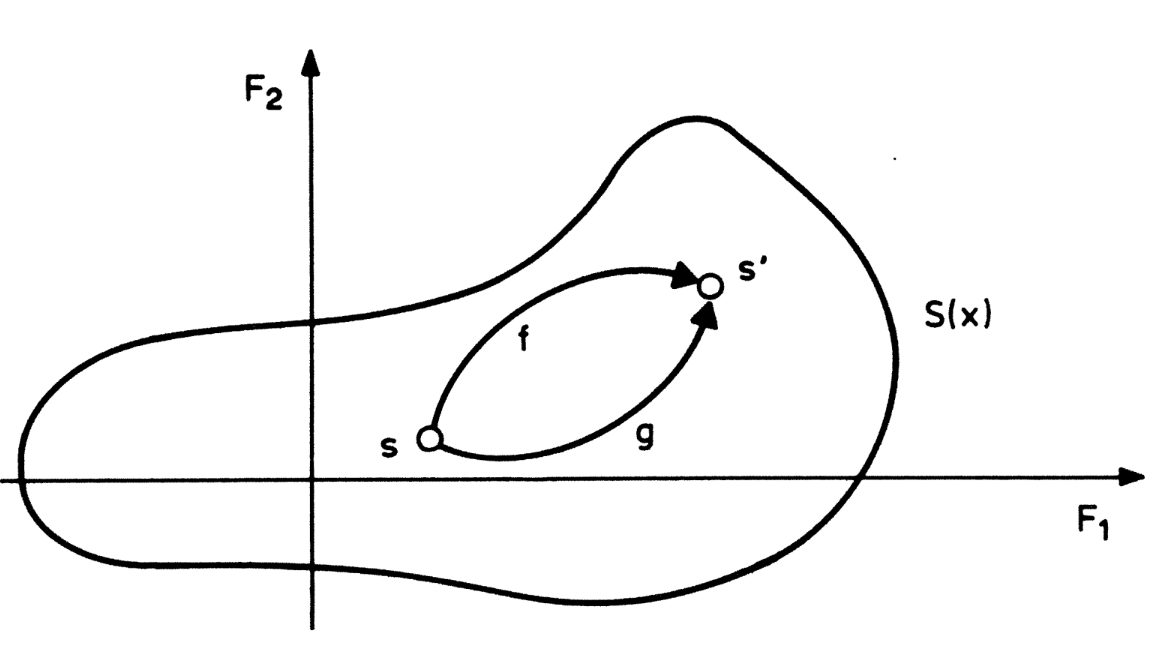
\includegraphics[width=0.9\textwidth]{img/Figura5-5.png}
		\\ \scriptsize Fig. 5.5. Dos procesos diferentes que dan lugar al mismo cambio neto.
	\end{center}
    curva g, donde g $\neq$ f,f, debemos representar los eventos completos, o procesos, mediante
las tripletas ordenadas $\langle s, s^{\prime}, f \rangle$ y $\langle s, s^{\prime}, g \rangle$ respectivamente. 
    Ahora bien, las funciones f y g que aparecen en nuestra ilustración (imaginaria) anterior
    no deben ser arbitrarias: deben ser legales si
    queremos permitir solo eventos legales y descartar todos los imposibles. En otras palabras, f y g deben ser leyes que posea la cosa
    x en cuestión o transformaciones del espacio de estados legales $Sl(X)$ compatibles
    con esas leyes. (Las funciones no tienen por qué ser funciones legales: pueden
    representar leyes objetivas junto con restricciones y circunstancias, como
    condiciones iniciales y condiciones límite, o pueden ser cambios de
    representación que dejen inalteradas todas las leyes de la cosa). Esto
    sugiere hacer
    
    DEFINICION 5.8 $S_{\mathbb{L}}(x)$ ser un espacio de estados legítimo para una cosa x. Entonces, la
familia de transformaciones legítimas del espacio de estados en sí mismo es el conjunto de
funciones
    \begin{center}
        $G_{\mathcal{L}}(x)=\{g \text{ is a function } |g:S_{\mathcal{L}}(x)\rightarrow S_{\mathcal{L}}(x)
        \text{ \& } g \text{ is compatible with the laws of } x\}$.
    \end{center}

    Claramente, la transformación de identidad $i_{S}: S_{\mathcal{L}}(x)\rightarrow S_{\mathcal{L}}(x)$, donde $i_{S}(s)=s$ por cada $s\in S_{\mathcal{L}}(x)$, es miembro fundador de $G_{\mathcal{L}}(x)$. No representa ningún cambio y puede componerse con cualquier transformación no trivial dada.

Cada una de estas transformaciones no triviales $g \in G_L(x)$, donde $g \neq i_S$, ayuda a representar una característica del cambio total experimentado por x, por ejemplo, su cambio de lugar, de población o de aglomeración. Dado que los cambios reales son multifacéticos, deben representarse con la ayuda de una serie de transformaciones diferentes que se combinan para formar el cambio total. Así, un evento termoeléctrico puede considerarse como la composición de un evento térmico y un evento eléctrico, pero no en el sentido de «composición».


    cubierta por la operación binaria * introducida en la sección 2.2. (La acepción
    de «composición» empleada en la presente sección se entiende mejor

    si se tiene en cuenta que $G_L(x)$ is a proper subset of $S_L(x)^{S_L(x)}$, i.e. the family of all the functions on $S_L(x)$ -- not just those representing lawful changes. But the wider set has the monoid structure, since the composition of any two transformations of $S_L(x)$ is a third transformation of the same set, and the latter includes the identity transformation.)
    
        Ahora pasemos al concepto de interés:
    
    \textbf{PRINCIPIO 5.3} Deja $S_L(x)$ ser un espacio de estado legítimo para una cosa $x$, y deja $G_L(x)$ ser la familia de transformaciones legales del espacio de estados    en sí mismo. Entonces, un evento (o proceso) legal con puntos finales $s$ and $s'$, donde $s, s' \in S_L(x)$, es representable como un triple $\langle s, s', g   \rangle$, donde $g \in G_L(x)$ y $s' = g(s)$.

    A esto lo llamamos el \emph{representación funcional del cambio}. Claramente, subsumirá la representación del par ordenado, que se obtiene cuando la transformación $g$ Claramente, subsumirá la representación del par ordenado, que se obtiene cuando la transformación

    ConConsideremos el caso paradigmático del modelo clásico de una partícula. El   estado dinámico instantáneo de tal cosa (modelo) moviéndose en una línea viene  dado por los valores instantáneos de la posición $q$ y el momento $p$ de la    partícula, considerados como variables independientes. El espacio de estados nomológico (llamado \emph{espacio de fase}) de tal cosa es un subconjunto del plano cartesiano. $\mathbb{R}^2$. La transformación que representa el movimiento puede calcularse siempre que se conozcan o se supongan $(a)$ las ecuaciones de movimiento y $(b)$ las fuerzas y restricciones que actúan sobre la partícula. Supongamos, para fijar ideas, que la fuerza que actúa sobre la partícula es elástica. En este caso, nuestro objeto es un oscilador lineal y sus leyes son las ecuaciones canónicas (o de Hamilton), que en este caso particular se reducen a
    \[
    \dot{q} = p/m, \quad \dot{p} = -kq,
    \]
    donde $m$ es la masa de la partícula y $k$ la constante elástica. Luego    llamando $q(t)=q$, $q(t+h)=q'$, donde $h \in \mathbb{R}^+$, y de manera similar para el momento, y expandiendo q' y p' en series de potencias, se obtiene

    \[
    \begin{aligned}
    q' &= q \cos ah + a^{-1}p \sin ah \\
    p' &= p \cos ah - aq \sin ah
    \end{aligned}
    , \text{ with } a = (k/m)^{1/2}.
    \]

    El valor $q'$ de la coordenada de posición en el momento $t$ + $h$ es entonces una función de los valores anteriores tanto de la posición como del momento, y
    lo mismo ocurre con el valor del momento $p'$. Una transformación que representa este cambio (movimiento) se denomina transformación canónica, o una transformación
    que satisface las ecuaciones canónicas del movimiento. Esta transformación,
    para un valor dado del desplazamiento temporal $h$, es una aplicación g:
    
    $\mathbb{R}^2 \to \mathbb{R}^2$ de tal manera que $g(q, p) = \langle q', p' \rangle$ como arriba. (Hay dos funciones involucradas, pero pueden considerarse simplemente como dos componentes de $g$.) La transformación puede considerarse como una rotación en el espacio de estados, donde los ejes cartesianos son ahora $x = a^{-1}p$ y $y=q$, y el ángulo de rotación $\alpha = ah$. y el ángulo de rotación. Esta transformación, lejos de ser arbitraria, está limitada por las leyes del movimiento. El efecto neto de esta restricción es que la elipse $p^2/a^2 + q^2 = 1$ se transforma en la elipse $p'^2/a^2 + q'^2 = 1$ en lugar de convertirse en una curva de otro tipo.

    A menos que el espacio de estados sea unidimensional, el cambio estará   representado por más de una función definida en el espacio de estados. Así, en el ejemplo anterior, la función de transformación resultó tener dos componentes, $u$ y $v$, de tal manera que $q' = u(q, p)$ y $p' = v(q, p)$. pero $u$  y $v$ son, como se ha señalado anteriormente, los dos componentes de una sola función $g$ cartografía $S(x)$ en sí mismo y satisfaciendo las ecuaciones de movimiento.
    
    \subsection{El espacio de los acontecimientos legales}

    In Sec. 2.2 Hemos caracterizado el espacio de eventos netos concebibles. Ahora pasamos a caracterizar el espacio de eventos realmente posibles. (i.e. lawful) eventos, teniendo en cuenta todos los estados intermedios entre los puntos finales que definen los eventos de red. Principio de recuerdo 5.3 en relación con la representación funcional de un proceso completo —no solo sus puntos finales— como un triple ordenado. $\langle s, s', g \rangle$. La recopilación de todos estos triples para una transformación fija. $g$ puede considerarse como un conjunto de pares ordenados y un subconjunto del espacio $E(x)$ de acontecimientos concebibles. Representa la totalidad de los cambios de tipo $g$ que ocurre en o a algo $x$. Y el espacio total de eventos para una cosa determinada es la colección de todos esos espacios de eventos parciales. Más explícitamente, proponemos

    \textbf{DEFINICION 5.9} Deja $S_L(x)$ ser un espacio de estado legítimo para una cosa $x$, y dejar $G_L(x) \subseteq S_L(x)^{S_L(x)}$ ser la familia de transformaciones legales de $S_L(x)$. Entonces
    (i) el $g$-transformaciones legales (o conjunto de\textit{cambios de tipo g})   for $x$, or \textit{espacio de sucesos g-legítimos} en $x$, es el conjunto de     pares ordenados de estados
    $E_g(x) = \{ \langle s, s' \rangle | s, s' \in S_L(x) \times S_L(x) | s' = g    (s) \ \& \ g \in G_L(x) \}$;
    (ii) el \textit{totalidad de las transformaciones legales} de $x$, o \textit    {espacio de eventos legales} (en todos los aspectos) en $x$, es la unión de     todos los espacios parciales de eventos:
    \[ E(x) = \bigcup_{g \in G_L(x)} E_g(x). \]

    (Podríamos haber definido $E_L(x)$ como la familia de todos $E_g(x)$'s, pero    entonces un evento singular perteneciente a cualquiera de los últimos no   pertenecería a los primeros.)

    Relajemos ahora la condición de que las transformaciones del espacio de     estados legales sean ellas mismas legales, y consideremos el espacio de     eventos concebibles. Ahora estamos en condiciones de generalizar el resultado   obtenido en la sección 2.2 relativo a los eventos netos. Consideremos los     eventos $\langle s, s', g \rangle$ y $\langle s', s'', h \rangle$, donde $s,    s', s'' \in S_L(x)$, y $g, h \in G(x) = S_L(x)^{S_L(x)}$. Es decir,    consideramos dos procesos concebibles que ocurren en una misma cosa. Debido a  las transformaciones $g$ y $h$ Es decir, consideramos dos procesos concebibles   que ocurren en una misma cosa. Debido a las transformaciones 
    \[ s \xrightarrow{g} s' \xrightarrow{h} s'' \]
    para producir el cambio neto $\langle s, s'', h \circ g \rangle$, donde     '$\circ$' significa composición de funciones. En el caso particular en que  $h=i_S$ (identity) obtenemos
    \[ s \xrightarrow{g} s' \xrightarrow{i_S} s' \]
    lo que se reduce a $\langle s, s', g \rangle$. Esto demuestra que el espacio    de los acontecimientos concebibles es una categoría. Más concretamente, lo     hemos demostrado con total generalidad.

    \textbf{TEOREMA 5.1} Deja $S_L(x)$ ser un espacio de estado legítimo para una   cosa $x$, and $G(x)=S_L(x)^{S_L(x)}$ la totalidad de (legal e ilegal)     transformaciones de $S_L(x)$. Además, dejemos que '$\circ$' designar la     composición de transformaciones (funciones) en $G$. Luego el triple $\mathcal   {C} = \langle S_L(x), G(x), \circ \rangle$, llamado el \textit{espacio     concebible de x}, es una categoría. Los objetos de esta categoría son todos     los estados. $s \in S_L(x)$ de la cosa, los morfismos, todas las    transformaciones $s \xrightarrow{g} s'$ con $g \in G(x)$ y $s' = g(s)$, y the  identidades las funciones $s \xrightarrow{i_S} s$.

    Este resultado (obtenido con la ayuda de Arturo Sangalli) no es muy     importante porque se refiere a la estructura del espacio de los acontecimientos concebibles  y no a la de los acontecimientos legales. Sin embargo, muestra la estructura en la que   el espacio de los acontecimientos legales $\mathscr{E}_L(x) = \langle S_L(x), G_L(x), \circ  \rangle$ está integrado. Además, nos enseña cómo componer eventos completos en lugar de solo eventos de red. De hecho, hemos aprendido que la composición de eventos se lleva a cabo tal y como indica

    \textbf{DEFINICION 5.10} Deja $S_L(x)$ ser un espacio de estado para una cosa $x$, Y   $G_L(x)$ el conjunto correspondiente de transformaciones legales de $S_L(x)$. Further,  llamada $e=\langle s, s', g \rangle$ and $e' = \langle s', s'', h \rangle$ dos eventos en el espacio legal para eventos $E_L(x)$ definido por $S_L(x)$ Y $G_L(x)$.  Entonces $e$ Y $e'$ \textit{compose} en el orden indicado para formar un tercer evento $e''$ si y solo si el final del primero coincide con el comienzo del segundo y si las dos transformaciones se componen para formar una tercera transformación legítima. Si la composición tiene lugar, entonces se dice que el primer evento\textit{preceder} el segundo. En símbolos:
    (i)
    \[
    \langle s, s', g \rangle * \langle s', s'', h \rangle =
    \begin{cases}
        \langle s, s'', h \circ g \rangle & \text{if } s' = s'' \text{ \& } h   \circ g \in G_L(x) \\
        \text{undefined} & \text{otherwise}
    \end{cases}
    \]
    (ii) $e < e' =_{df} e * e' \in E_L(x)$.

    Y ahora algunas ilustraciones atrasadas.

    \textbf{Ejemplo 1} Supongamos que se trata de un sistema conservativo con $n$ componentes.  Su espacio de estados clásico es el espacio cartesiano de dimensión $6n$ generado por     la función de estado cuyos componentes son las $3n$ coordenadas de posición generalizadas   y los $3n$ momentos. El espacio de sucesos está incluido en el conjunto de   gráficos de las transformaciones canónicas o de contacto, que son aquellas   transformaciones del espacio de estados (fase) que dejan invariantes las leyes del movimiento . Para más detalles sobre el caso más simple, véase el ejemplo de la sección 2.3.
    \textbf{Ejemplo 2} El espacio de estados de un sistema cuántico-mecánico es un espacio de Hilbert, es decir, un conjunto determinado de funciones. El operador $T = \exp(iHt/\hbar)$ definido en este espacio, es decir, $T: S \to S$, permite representar los cambios en los estados del sistema. Por lo tanto, si $Q(t_0)$ representa el valor de una propiedad $Q$    del sistema en el momento $t_0$, entonces su valor en el momento $t$ es $Q(t) = TQ(t_0)T^   {-1}$.
    \textbf{Ejemplo 3} Algunos o incluso todos los componentes de la función de estado  para una cosa podrían ser variables aleatorias. Entonces, el espacio de estado correspondiente   sería un espacio de estado probabilístico (cap. 4, sec. 4.2). Las leyes del cambio, o  al menos algunas de ellas, no se referirían a los estados de manera directa, sino   más bien a sus probabilidades o, mejor dicho, a las probabilidades de las diversas  transiciones de estado posibles (legítimas). Estas probabilidades son condicionales.  Consideremos el caso simple de un espacio de estado con un número finito de puntos, cada uno de los cuales tiene una probabilidad definida. Cada estado final $s_f$ puede surgir (originarse) a partir de cualquier otro estado $s_i$ con una probabilidad definida $\Pr(s_f|s_i)$, que por supuesto puede ser nula para algunos pares de estados. Para un $i$ fijo, todas estas probabilidades suman la unidad. La probabilidad total de que se actualice un estado $s_f$ es
  \[
  \Pr(s_f) = \sum_i \Pr(s_i) \cdot \Pr(s_f|s_i).
  \]

  \subsection*{2.5. Seguimiento de los estados cambiantes}
  Mientras que algunas propiedades de una cosa, como su composición, son invariables o absolutas, otras, como su energía, dependen del marco o son relativas. Dado que todas las cosas poseen energía, los estados de todas las cosas son relativos: recuerde el capítulo 3, sección 2.8. Y como los estados son relativos, también lo son los acontecimientos. Es cierto que acontecimientos como encender un interruptor o besar parecen absolutos. Pero esto se debe únicamente a que, al pensar en ellos, nos centramos en lo que parece típico, dejando de lado una serie de características que dependen del marco, como la ubicación y la velocidad de la(s) cosa(s) en la(s) que se producen los acontecimientos. Una descripción razonablemente completa de un acontecimiento requiere la determinación de una serie de rasgos, la mayoría de los cuales están destinados a ser relativos más que absolutos. Por lo tanto,

  \textbf{RULE 6.1} Referir cada función de estado es decir, cada espacio de estado y cada espacio de eventos— a algún elemento estándar (marco de referencia) u otro.

  La referencia explícita a los estándares no solo sirve como recordatorio de que el cambio es relativo: también puede utilizarse para etiquetar estados y realizar un seguimiento de ellos de una forma más precisa que hasta ahora. De hecho, este es el objetivo de la Definición 3.14: nos permite identificar los estados de las cosas en términos de estados de referencia o estados de un estándar. Recordemos cómo se hizo esto y mejoremos esa parametrización.
  Sea $S(f)$ un espacio de estados de un marco de referencia $f$ para un objeto $x$ con espacio de estados $S(x)$. Además, supongamos que el dominio de la función de estado $F$ que abarca $S(x)$, lejos de no estar relacionado con el marco de referencia, es igual a la colección $S(f)$ de estados de referencia. Es decir, establezcamos $F: S(f) \to S(x)$, de modo que cada estado de referencia $t \in S(f)$ se empareje con un único estado de cosa $s=F(t) = \langle F_i(t)| 1 \le i \le n \rangle$, donde $n$ es el número de propiedades representadas por $F$. La función de estado $F$ es ahora la lista de propiedades de la cosa $x$ \textit{relativa a} (o parametrizada por) los estados del marco de referencia $f$. Dado cualquier estado de referencia $t$, $F$ elige el estado de cosa correspondiente $F(t)$. Y una sustitución de puntos, cada uno de los cuales tiene una probabilidad definida. Cada estado final $s_f$ puede surgir (originarse) de cualquier otro estado $s_i$ con una probabilidad definida $\Pr(s_f|s_i)$, que por supuesto puede ser nula para algunos pares de estados. Para un $i$ fijo, todas estas probabilidades suman la unidad. La probabilidad total de que se actualice un estado $s_f$ es
  \[
  \Pr(s_f) = \sum_i \Pr(s_i) \cdot \Pr(s_f|s_i).
  \]

  \subsection*{2.5. Seguimiento de los estados cambiantes}

  Mientras que algunas propiedades de una cosa, como su composición, son invariables o absolutas, otras, como su energía, dependen del marco o son relativas. Dado que todas las cosas poseen energía, los estados de todas las cosas son relativos: recuerde el capítulo 3, sección 2.8. Y como los estados son relativos, también lo son los acontecimientos. Es cierto que acontecimientos como encender un interruptor o besar parecen absolutos. Pero esto se debe únicamente a que, al pensar en ellos, nos centramos en lo que parece típico, dejando de lado una serie de características que dependen del marco, como la ubicación y la velocidad de la(s) cosa(s) en la(s) que se producen los acontecimientos. Una descripción razonablemente completa de un acontecimiento requiere la determinación de una serie de rasgos, la mayoría de los cuales están destinados a ser relativos más que absolutos. Por lo tanto.

  \textbf{RULE 6.1} Referir cada función de estado es decir, cada espacio de estado y cada espacio de eventos— a algún elemento estándar (marco de referencia) u otro.

  La referencia explícita a los estándares no solo sirve como recordatorio de que el cambio es relativo: también puede utilizarse para etiquetar estados y realizar un seguimiento de ellos de una forma más precisa que hasta ahora. De hecho, este es el objetivo de la Definición 3.14: nos permite identificar los estados de las cosas en términos de estados de referencia o estados de un estándar. Recordemos cómo se hizo esto y mejoremos esa parametrización.

  Sea $S(f)$ un espacio de estados de un marco de referencia $f$ para un objeto $x$ con espacio de estados $S(x)$. Además, supongamos que el dominio de la función de estado $F$ que abarca $S(x)$, lejos de no estar relacionado con el marco de referencia, es igual a la colección $S(f)$ de estados de referencia. Es decir, establezcamos $F: S(f) \to S(x)$, de modo que cada estado de referencia $t \in S(f)$ se empareje con un único estado de cosa $s=F(t) = \langle F_i(t)| 1 \le i \le n \rangle$, donde $n$ es el número de propiedades representadas por $F$. La función de estado $F$ es ahora la lista de propiedades de la cosa $x$ \textit{relativa a} (o parametrizada por) los estados del marco de referencia $f$. Dado cualquier estado de referencia $t$, $F$ elige el estado de cosa correspondiente $F(t)$. Y una sustitución de
  puntos, cada uno de los cuales tiene una probabilidad definida. Cada estado final
  $s_f$ puede surgir (tener su origen) en cualquier otro estado $s_i$ con una probabilidad definida $\Pr(s_f|s_i)$, que, por supuesto, puede ser nula para algunos pares de estados. Para un $i$ fijo, todas estas probabilidades suman la unidad. La probabilidad total de que se actualice el estado $s_f$ es
  \[
  \Pr(s_f) = \sum_i \Pr(s_i) \cdot \Pr(s_f|s_i).
  \]

  \subsection{Seguimiento de los estados cambiantes}

  Mientras que algunas propiedades de una cosa, como su composición, son invariables o absolutas, otras, como su energía, son
  dependientes o relativas. Dado que todo posee energía, los estados de todo son relativos: recuerde el capítulo 3, sección 2.8. Y como los estados son
  relativos, también lo son los acontecimientos. Es cierto que acontecimientos como encender un interruptor o besar
  parecen absolutos. Pero esto es solo porque al pensar en ellos nos centramos en lo que parece típico, dejando de lado una serie de características que dependen del marco, como la ubicación y la velocidad de la(s) cosa(s) en la(s) que ocurren los eventos. Una descripción razonablemente completa de un evento requiere la determinación de una serie de rasgos, la mayoría de los cuales están destinados a ser relativos en lugar de absolutos. Por lo tanto

  \textbf{RULE 6.1} Remitir todas las funciones estatales - Por lo tanto, cada espacio de estados y cada espacio de eventos se relaciona con algún estándar (marco de referencia) u otro.

  La referencia explícita a los estándares no solo sirve como recordatorio de que el cambio es relativo: también puede utilizarse para etiquetar estados y realizar un seguimiento de ellos de una forma más precisa que hasta ahora. De hecho, este es el objetivo de la Definición 3.14: nos permite identificar los estados de las cosas en términos de estados de referencia o estados de un estándar. Recordemos cómo se hizo esto y mejoremos esa parametrización.

  Sea $S(f)$ un espacio de estados de un marco de referencia $f$ para un objeto $x$ con espacio de estados $S(x)$. Además, supongamos que el dominio de la función de estado $F$ que abarca $S(x)$, lejos de no estar relacionado con el marco de referencia, es igual a la colección $S(f)$ de estados de referencia. Es decir, establezcamos $F: S(f) \to S(x)$, de modo que cada estado de referencia $t \in S(f)$ se empareje con un único estado de cosa $s=F(t) = \langle F_i(t)| 1 \le i \le n \rangle$, donde $n$ es el número de propiedades representadas por $F$. La función de estado $F$ es ahora la lista de propiedades de la cosa $x$ \textit{relativa a} (o parametrizada por) los estados del marco de referencia $f$. Dado cualquier estado de referencia $t$, $F$ elige el estado de cosa correspondiente $F(t)$. Y una sustitución de

  un marco no equivalente $f'$ para el marco $f$ irá acompañado de diferentes valores $F(t')$ de la función de estado.

  Los estados de un marco de referencia pueden describirse con diversos grados de precisión. Pero si vamos a utilizarlos para etiquetar o identificar estados de cosas, entonces esa precisión no debe ser inferior a la empleada para describir los estados de las cosas. Ahora bien, en ciencia se suele buscar, y a menudo se alcanza, la máxima precisión, que en este caso consiste en asignar valores reales a las propiedades individuales de las cosas. Es decir, en la mayoría de los casos, cada valor de la función de estado $F_i$ para una cosa dada es igual a un número real $r_n$, de modo que el estado de la cosa en (\textit{relativo a}) $t \in S(f)$ es $F(t) = \langle F_i(t)| 1 \le i \le n \rangle = \langle r_1, r_2, \dots, r_n \rangle$. Un grado tan alto de precisión exige una precisión similar en la descripción de los estados de referencia. Y esa precisión se consigue coordinándolos, es decir, asignándoles valores de coordenadas.

  El procedimiento de coordinatización se visualiza mejor interpretando $S(f)$ como un sistema de cuatro ejes cartesianos, de modo que a cada estado de referencia se le asigna un cuádruple de números reales. Es decir, seleccionamos aquellas propiedades de un marco de referencia que pueden representarse en una cuadrícula de cuatro dimensiones, dejando de lado todas las demás propiedades. (Los puntos de la cuadrícula se interpretan finalmente como puntos en el espacio-tiempo). Por último, nos referimos a los estados de las cosas no en relación con los estados de referencia, sino con sus etiquetas numéricas. - Cuando decimos $'X$ estaba soñando en la esquina de la calle en 7:00 p.m.'. Es decir, emparejamos cada estado de cosa con un punto en la cuadrícula de referencia.

  La coordinatización de los estados de referencia se efectúa mediante una correspondencia uno a uno. $k: \mathbb{R}^4 \to S(f)$ entre cuádruples ordenadas de números reales y estados de referencia. La composición $\lambda = F \circ k$ de la función de coordinatización con la función de estado coincide con cada punto $r = \langle t, x, y, z \rangle$ en la cuadrícula de referencia con un estado de cosa $s$, i.e. $r \xrightarrow{k} t \xrightarrow{F} s$, como se muestra en la figura 5.6 y en el diagrama conmutativo de la página siguiente.

  Ahora, la cuadrícula de referencia está parcialmente ordenada. De hecho, si $r$ y $s$ son cuádruples de números reales, entonces $r \le s$ si y solo si cada componente o coordenada de $r$ es menor que la coordenada correspondiente de $s$. Es decir,
  \[
  \langle r_1, r_2, r_3, r_4 \rangle \le \langle s_1, s_2, s_3, s_4 \rangle \text{ iff } r_i \le s_i \text{ for all } i=1, 2, 3, 4.
  \]
  En consecuencia $\langle S(f), \le \rangle$ es un conjunto parcialmente ordenado. Este orden no está conectado: no todos los pares de estados de referencia están relacionados por $\le$: véase la figura 5.7. Y se impone el mismo tipo de orden, a través de $F$, en el plató $S(x)$ de cosa.

    \begin{center}
      \includegraphics[width=0.9\textwidth]{img/Figura5-6.png}
      \\ \scriptsize Fig. 5.6. Coordinatización de estados. Cada estado de referencia $t \in S(f)$ se asigna como máximo un estado de cosa $s \in S(x) \subseteq \mathbb{R}^n$ y está representado por un cuádruple de números reales $r \in \mathbb{R}^4$.
    \end{center}

    \begin{center}
      \includegraphics[width=0.9\textwidth]{img/Figura5-7.png}
      \\ \scriptsize Fig. 5.7. El estado $s$ precede a todos los demás en la región sombreada, pero a ninguno fuera de esta.
    \end{center}

      estados incluso si $F$ dno toma valores en $\mathbb{R}^n$ - como cuando se dice que un mamífero pasa por cuatro etapas de desarrollo.

      Las consideraciones anteriores pueden resumirse en

      \textbf{DEFINITION 5.11} deja $f$ ser un marco de referencia para algo $x$ y deja $S(f)$ y $S(x)$ sean los respectivos espacios de estados. Además, supongamos que $S(f)$ es

      recorrido por una función de estado de cuatro componentes, mientras que $S(x)$ es explorado por una función de estado de $n$-componentes $F$. Entonces, una \textit{coordenadización de los estados} tanto de $x$ como de $f$ es una correspondencia biunívoca $k: \mathbb{R}^4 \to S(f)$ tal que
  (i) $k$ asigna a cada estado de referencia $s \in S(f)$ una cuádrupla de números reales $r$ - como consecuencia de lo cual cada estado del ente $s \in S(x)$ se identifica como la $n$-tupla $s = (F \circ k)(r)$;
  (ii) $k$ preserva el orden, es decir, el orden parcial de $\mathbb{R}^4$ induce a través de $k$ el ordenamiento parcial de los estados de referencia, lo que a su vez ordena los estados del ente: para todo $t_1, t_2 \in S(f)$,
  \begin{quote}
      si $r_1 \le r_2$ entonces $k(r_1) \le k(r_2) \text{ y } F(t_1) \le F(t_2)$,
      donde \quad $t_i = k(r_i)$.
  \end{quote}
  En otras palabras, una coordenadización de estados es una función que preserva el orden, etiquetando y ordenando los estados del ente a través de los estados de referencia:
  \[
  \langle\mathbb{R}^4, \le\rangle \xrightarrow{k} \langle S(f), \le\rangle \xrightarrow{F} \langle S(x), \le\rangle.
  \]
  A medida que el marco de referencia pasa de un estado a otro, también lo hace el ente: los estados sucesivos de un ente pueden entonces ser asociados y, por lo tanto, identificados por (no \textit{con}) los estados sucesivos del estándar. Y a su vez, el ordenamiento de los estados induce un ordenamiento de los eventos (en el mismo ente y relativo al mismo marco). Por consiguiente, podemos establecer

  \textbf{DEFINICIÓN 5.12} Sean $s, s', s'', s'''$ cuatro estados de un ente dado relativos a un cierto marco de referencia, tal que los dos primeros forman un evento neto $e = \langle s, s' \rangle$ y los dos últimos otro evento $e'=\langle s'', s''' \rangle$. Entonces
  (i) $e \le e' =_{df} s \le s'' \text{ y } s' \le s'''$.
  (ii) $e \sim e' =_{df} e \le e' \text{ y } e' \le e$.
  La relación $\le$ de orden de eventos es reflexiva; dos eventos son congruentes si y solo si sus estados iniciales y finales correspondientes son congruentes, es decir,
  \[
  e \sim e' =_{df} s \sim s'' \text{ y } s' \sim s'''.
  \]
  Es claro también que $\le$ es antisimétrica y transitiva. Por lo tanto, $\le$ es un orden parcial - a diferencia de la relación introducida en la Definición 5.7, que era solo un orden parcial estricto. Por lo tanto, en lugar del Corolario 5.5 tenemos

  \textbf{COROLARIO 5.6} Para todo ente $x$ y relativo a cualquier marco de referencia dado, $\langle E(x), \le \rangle$ es un conjunto parcialmente ordenado.

  \bigskip

    Nuestra nueva definición de orden de eventos es más completa 
    que la Definición 5.7, ya que incluye el caso particular cuando $e$ 
    se compone con $e'$ para formar un tercer evento $e'' = e * e'$ (en cuyo caso 
    $s' = s''$), así como el caso en que no se componen. (Véase la Figura 5.8.) La 
    composición de eventos solo es posible si la precedencia es apropiada:
    $e * e' = e''$ si y solo si $s' = s''$ y $e < e'$.

    \begin{center}
        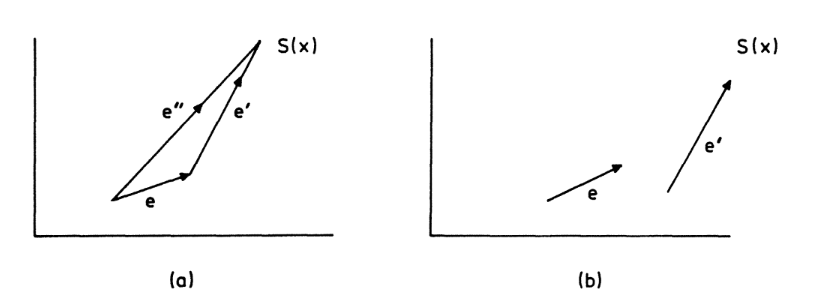
\includegraphics[width=0.6\textwidth]{img/Figura5-8.png}
        \\ \scriptsize Fig. 5.8. Orden de eventos. (a) $e < e'$ y 
        ambos se componen para formar $e''$. (b) $e < e'$ pero no se componen.
    \end{center}

    \noindent En consecuencia, dos eventos no se componen si ninguno precede al otro.
    Lo cual es bastante obvio, ya que se supone que los eslabones de una cadena 
    de eventos se suceden. Esto, a su vez, invita a definir una cadena de eventos 
    como un conjunto numerable y estrictamente parcialmente ordenado de eventos $E^*(x)$ 
    incluidos en el espacio de eventos de un evento $x$ tal que, para cualquier $e, e' \in E^*(x)$, 
    si $e < e'$, entonces el estado final de $e$ coincide con el estado inicial de $e'$, de modo que 
    ambos eventos se componen. Más sobre esto en la sección 3.1.

    Finalmente, procederemos a formalizar la noción de una colección variable, es decir, una cuya pertenencia 
    cambia a medida que los estados de referencia se suceden, por ejemplo, la población de una ciudad. Obviamente, 
    el concepto de conjunto no es válido, ya que cada conjunto tiene una pertenencia fija. Pero en lugar de usar un 
    solo conjunto, podemos emplear una familia de conjuntos indexados por un parámetro de cambio, llamémoslo $t$. 
    Así, llamando $C_t$ a una colección en $t$, formamos la familia $C=\{C_t | t \in \Omega\}$, que puede llamarse 
    una colección variable. O, equivalentemente, podemos proponer

    \bigskip

    \noindent DEFINICIÓN 5.13 Sea $t \in S(f)$ el parámetro de cambio del marco $f$. Entonces cualquier función
    \begin{center}
        $K: S(f) \to C$, con $C=\{C_t | t \in S(f)\}$,
    \end{center}
    tal que $K(t) = C_t$, para $t \in S(f)$, se llama una \textit{colección variable}.

    \newpage

    Esta interpretación de una colección variable será adoptada de aquí en adelante, particularmente en el Vol. 4 de 
    este tratado, al tratar con poblaciones de moléculas, organismos o personas, cuya composición, a diferencia de la 
    de un conjunto, cambia en el tiempo. Es particularmente ventajoso para analizar propiedades de colecciones. Tómese, 
    por ejemplo, la numerosidad o población de una colección variable como un ecosistema. Puede ser considerada como una
    función $p: C \to \mathbb{N}$ que asigna a cada miembro de la familia $C$ un número natural $n \in \mathbb{N}$. Esta 
    función se compone con $K$ para producir la función $f = p \circ K: S(f) \to \mathbb{N}$, la cual asigna a cada estado 
    de referencia (o instante) $t \in S(f)$ un número natural, a saber, la población de la colección variable. (Para tiempos 
    discretos, la teoría matemática de conjuntos a través del tiempo está disponible.)

    \subsection{\textit {Tasa, Alcance y Potencial de Cambio}}

    \noindent Una primera noción que queremos aclarar es la de tasa de cambio. En realidad, existe una gran familia de conceptos 
    de tasa de cambio, de los cuales presentaremos solo los dos más comunes.

    Supongamos que tanto los estados de referencia como los estados de la cosa han sido debidamente coordinados (Secc. 2.5). Cada 
    estado de referencia $t \in S(f)$ es entonces representado por un cuádruple de números reales: $t = (\alpha, \beta, \gamma, \delta)$. 
    En consecuencia, el estado de la cosa correspondiente es $s = \mathbb{F}(t) = \mathbb{F}(\alpha, \beta, \gamma, \delta)$. Si $\mathbb{F}$ 
    tiene un componente $F_i$ que es una vez derivable con respecto a uno de los cuatro parámetros de referencia, digamos $\alpha$, entonces 
    la tasa de cambio de $F_i$ con respecto a $\alpha$ es la derivada parcial de $F_i$ con respecto a $\alpha$. La cosa no cambia en absoluto 
    en el $i$-ésimo aspecto sobre el intervalo $[\alpha_1, \alpha_2]$ si y solo si $\partial F_i/\partial \alpha = 0$ para todo $\alpha \in [\alpha_1, \alpha_2]$. 
    Cambia rápidamente en el mismo aspecto sobre el mismo intervalo si la tasa de cambio correspondiente es apreciable con relación a la 
    propia $F_i$; de lo contrario, cambia lentamente. No hace falta decir que el parámetro de referencia puede ser, pero no necesariamente 
    tiene que ser, el tiempo. En resumen, podemos establecer:

    DEFINICIÓN 5.14 Sean los estados de una cosa $x$ coordinados a través de los de un cierto marco de referencia, de modo que cada estado de la cosa es de la forma $s=\mathbb{F}(\alpha, \beta, \gamma, \delta)$, donde los argumentos son los parámetros que identifican los estados de referencia. Además, sea el $i$-ésimo componente de $\mathbb{F}$ derivable con respecto a $\alpha$. Entonces
    \begin{itemize}
        \item[(i)] la \textit{tasa de cambio relativa} de $x$ en el $i$-ésimo aspecto y con respecto a $\alpha$ es
            \[
                V_i = \frac{1}{F_i} \frac{\partial F_i}{\partial \alpha}.
            \]    
        \item[(ii)] \textit{la magnitud relativa del cambio} de $x$ en el aspecto i-ésimo, con respecto a a y en el intervalo , es
        \begin{center}
            $
                \Delta_i(\alpha_1, \alpha_2) = \frac{\ln F_i(\alpha_2) - \ln F_i(\alpha_1)}{\alpha_2 - \alpha_1}
                \text{proporcionado } F_i(\alpha_1), F_i(\alpha_2) > 0.
            $
        \end{center} 
    \end{itemize}

    Si la cosa cambia periódicamente con un periodo [$a_1$,$a_2$], la magnitud de su
    cambio a lo largo de un múltiplo entero del periodo es nula. Esto proporciona una
    definición del concepto de \textit{cambio cíclico}.

    La definición anterior no sirve en el caso de un espacio de estados probabilísticos 
    cuyos puntos no están emparejados con ningún marco de referencia. En este caso, nos interesan 
    los cambios globales que son invariables con respecto al marco. La tasa de cambio del estado $s_i$ 
    al estado $s_j$ puede considerarse como la probabilidad condicional de $s_j$ dado que $s_i$ se ha actualizado, 
    es decir, $Pr(s_j|s_i)$. El razonamiento detrás de esta elección es el siguiente. Pensemos en un objeto 
    complejo, cuyos $n_i$ componentes se encuentran en el estado $s_i$, $n_j$ en el estado $s_j$, y así sucesivamente. 
    Entonces, $niPr(s_j|s_i)$ medirá el número más probable de componentes que saltan del estado $s_i$ al estado $s_j$. 
    Cuanto mayor sea este producto, mayor será la tasa de cambio. La matriz estocástica $\lVert Q_{ij} \rVert = \lVert Pr(s_j|s_i) \rVert$
    representa entonces la tasa global de cambio de la cosa. Si la matriz es diagonal, es decir, si $Pr(s_j|s_i) = \delta _{ij}p_i$, 
    donde $\delta _{ij}$ es el delta de Kronecker y $p_i$ la probabilidad del estado $s_i$, entonces la cosa no cambia. Cuanto mayor es 
    el cambio, mayores son los términos fuera de la diagonal correspondientes de $\lVert Q_{ij} \rVert$. Y la magnitud del 
    cambio, también llamada \textit{movilidad}, es igual a la suma de los productos de los términos fuera de la diagonal 
    por sus contrapartes simétricas. Comprimimos todo esto en

    \noindent DEFINICIÓN 5.15 Sea $\langle S(x), Pr \rangle$, donde $S(x)$ es un espacio de estados numerable
    para una cosa $x$, y $Pr$ una medida de probabilidad en $S(x)$, un campo de posibilidades
    para $x$. Entonces 
    \begin{itemize}
        \item[(i)] la \textit{tasa global de cambio} de $x$ es la matriz estocástica
        \[
            \lVert Q_{ij}\rVert=\lVert Pr(s_j|s_i)\rVert \quad \text{con} \quad s_i,s_j\in S(x),
        \]
    \end{itemize}
    donde $Pr(s_j|s_i)$ es la probabilidad del estado $s_j$ dado que el estado $s_i$ se ha
    actualizado;
    \begin{itemize}   
        \item[(ii)] el \textit{grado de cambio (o movilidad)} de $x$ es
        \scriptsize
        \[
            \Delta = \sum_{i \ne j} Q_{ij} \cdot Q_{ji} = \sum_{i \ne j} Pr(s_j|s_i) \cdot Pr(s_i|s_j).
        \]
    \end{itemize} 

    Esta última es una medida de la variabilidad de ciertas cosas en ciertos aspectos, concretamente aquellas que pueden describirse con la 
    ayuda de campos de posibilidades enumerables. Pero no es una medida de la variabilidad global de una cosa arbitraria. ¿Qué tan cambiante 
    (en todos los aspectos) es una cosa arbitraria? De manera equivalente: ¿qué tan grandes son los espacios de eventos? Para responder a esta 
    pregunta (imprecisa), consideremos el conjunto de todas las propiedades de cualquier cosa real y un modelo teórico realista de dicha cosa, 
    por ejemplo, la teoría relativista del electrón o del campo gravitacional. Dicho modelo, o esquema funcional, se basa en un determinado conjunto 
    en el que se define una función de estado $\mathbb{F}$ de $n$ componentes, cada uno de los cuales representa una propiedad (cambiable) de la cosa. Al menos 
    algunos de los componentes de la función de estado están obligados a ser continuos con respecto a algunas de las "variables independientes". 
    Llamemos $\mathbb{F}$ a cualquier variable de estado continua de este tipo. A medida que la cosa cambia, los valores de $\mathbb{F}$ varían continuamente (o al menos de 
    forma continua por tramos), incluso si los de algunos otros componentes de $\mathbb{F}$ cambian por saltos. (Pensemos en una cosa que gana o pierde cuantos 
    de carga eléctrica, o en personas que ganan o pierden impulso). Véase la figura 5.9. Es evidente que el espacio (de estado) abarcado por $\mathbb{F}$ es innumerable.

    \begin{center}
        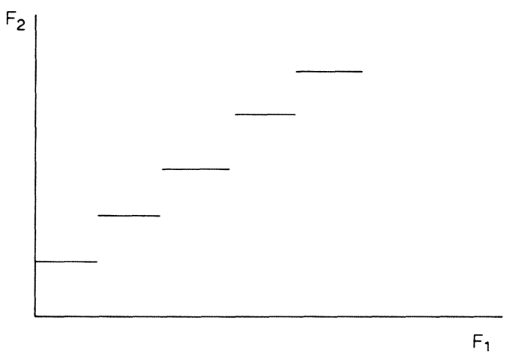
\includegraphics[width=0.4\textwidth]{img/Figura5-9.png}
        \\ \scriptsize Fig. 5.9. Un espacio de estados con un eje continuo ($F_1$) y otro discontinuo ($F_2$). La
        línea discontinua representa la evolución de la cosa. La totalidad de los estados es innumerable.
    \end{center}

    Suponemos que cada cosa tiene al menos una propiedad que cambia continuamente con respecto a una variable u otra, siendo la "variable independiente" normalmente una coordenada temporal o una coordenada espacial:
    
    \bigskip
    \noindent POSTULADO 5.2 Toda función de estado [realista] tiene al menos un componente continuo.

    \bigskip
    Dado que un espacio de estados es el conjunto de puntos explorados por la punta de la función de estado, tenemos que
    
    \bigskip
    \noindent COROLARIO 5.7 Todo espacio de estados [realista] es innumerable. Y a partir de la forma en que se construyen los eventos, también inferimos que

    \bigskip
    \noindent COROLARIO 5.8 Todo espacio de sucesos [realista] es innumerable.

    Es cierto que a menudo construimos modelos de cosas (objetos modelo) cuyos espacios de estados son numerables o incluso finitos. Pero esto se hace por conveniencia 
    más que por verdad, es decir, porque solo nos interesan algunos aspectos del conjunto. Por lo tanto, aunque la teoría de autómatas modela ciertas máquinas como si 
    tuvieran solo un número finito de estados, el diseño y la construcción reales de dichas máquinas presuponen teorías que implican espacios de estados no numerables, 
    como los analizados en el capítulo 3, secciones 2.4 y 2.5. Incluso si el universo consistiera solo en dos cosas en movimiento relativo (por ejemplo, una molécula diatómica), 
    el espacio de eventos del mundo sería no numerable. En conclusión, los espacios de eventos realistas son tan grandes como cualquier subconjunto de la recta real: 
    todos tienen el poder del continuo.

    Dado que todos los espacios de eventos realistas son igualmente voluminosos (Corolario 5.8), no proporcionan una medida adecuada del potencial de cambio de las cosas reales. 
    Debemos buscar esa medida en otra parte. Si examinamos las ciencias empíricas en busca de una propiedad que compartan todas las cosas, independientemente de su tipo y relacionada 
    con su capacidad de cambio, solo encontramos una propiedad universal: la energía. Además, la energía tiene la propiedad de que cuanto más compleja es la cosa, mayor es su potencial de 
    cambio. De hecho, la energía es estrictamente aditiva para las cosas que no interactúan, es decir, cuando el espacio de estados total del compuesto es igual a la unión de los espacios de 
    estados parciales (recuerde el capítulo 3, sección 2.7). Por lo tanto, hacemos

    \noindent POSTULADO 5.3 Existe exactamente una propiedad que poseen todas las cosas, la cual es aditiva para los agregados de cosas compuestas por partes separadas. Es decir, 
    si $\Theta$ es la clase de las cosas y $F$ la de los marcos de referencia, entonces existe una y solo una función de valor real $\varepsilon: \Theta \times F \to \mathbb{R}$ 
    tal que, para cualquier $x$ e $y$ en $\Theta$ tal que $x|y$,
    \[
        \varepsilon(x+y,f) = \varepsilon(x,f) + \varepsilon(y,f) \quad \text{para todo } f \in F.
    \]

    \noindent Esta función $\varepsilon$ se denomina \textit{energía}, y su valor en $(x, f)$ —es decir, \textit{la energía de x con respecto a f}— mide la \textit{variabilidad de x con respecto a f}.

    (La \textit{energeia} era un concepto ontológico antes de ser absorbido y transformado por la física moderna. A veces todavía se considera una noción metafísica, aunque por razones erróneas, concretamente 
    porque no representa una propiedad perceptible. El concepto general de energía es una noción ontológica genuina por una razón diferente, concretamente porque designa una propiedad universal. Por esta razón, 
    aparece en todas partes en la ciencia, aunque en algunas áreas, en particular la geografía y la historia, solo ha entrado recientemente. En cualquier caso, es agradable ver que el concepto de energía vuelve 
    al ámbito filosófico. Como ahora entendemos que la energía es una propiedad de las cosas, no hay peligro de que se reifique, y mucho menos de que se convierta en lo único existente, como hicieron los energistas 
    de principios de siglo, por ejemplo, Ostwald en 1902).

    Se podría objetar que el Postulado 5.3 no es lo suficientemente preciso para definir el concepto de energía. A esto se podría responder, en primer lugar, que la ciencia no proporciona una definición del concepto 
    general de energía. En segundo lugar, para un físico, el Postulado 5.3 es suficiente para \textit{identificar} $\varepsilon$ como la función de energía, ya que es la única propiedad cuantitativa (y aproximadamente aditiva) que tienen 
    todas las cosas. (En el caso de las cosas con partes que interactúan, la energía es ligeramente subaditiva). Todo lo que afirma nuestro axioma es que \textit{todas las cosas tienen energía}. No proporciona un método para 
    calcular la energía de ninguna cosa en particular: esa es una tarea de la ciencia. Y ninguna ciencia puede llevar a cabo esta tarea sin información precisa (o conjeturas) sobre el tipo de cosa, su estructura, sus 
    interacciones y sus circunstancias.

    Se pueden concebir ciertas propiedades que se presentan en grados infinitos. Por ejemplo, si el universo es infinito en extensión, entonces hay cosas que están infinitamente distantes unas de otras. Por otro lado, la energía de una parte 
    finita del universo se considera normalmente finita. (Es cierto que tanto en la física clásica como en la cuántica hay teorías que contienen teoremas —nunca axiomas— según los cuales ciertas cosas, como los electrones y las ondas 
    electromagnéticas planas, tienen energías infinitas. Sin embargo, estas fórmulas se consideran imperfecciones de las teorías, no de la naturaleza, y se recurre a varios trucos para evitarlas). Por lo tanto, estamos justificados al adoptar

    \bigskip
    \noindent POSTULADO 5.4 La energía de cualquier cosa compuesta por un número finito de cosas, y relativa a cualquier marco de referencia, es finita.

    Una consecuencia importante de la energía finita (o potencial de cambio) de todo lo finito es que el ritmo y el alcance de cada cambio son limitados. (Véase la figura 5.10.) Por ejemplo, la velocidad de un
    \begin{center}
        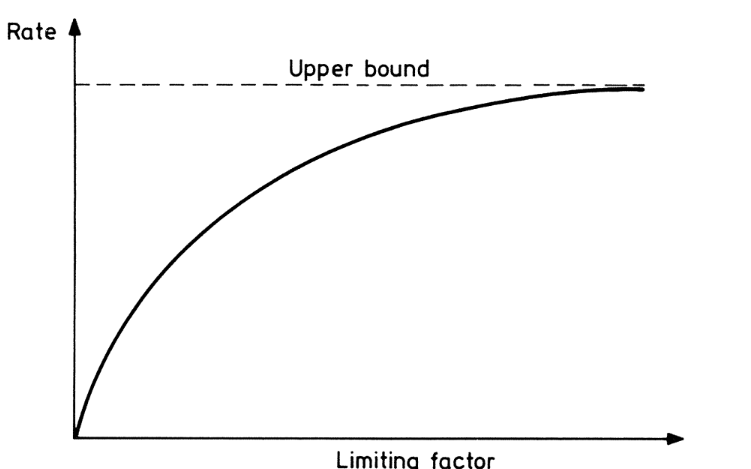
\includegraphics[width=0.6\textwidth]{img/Figura5-10.png}
        \\ \scriptsize Fig. 5.10. Relación entre la velocidad del proceso y la intensidad (o concentración) de un "factor limitante", como la energía.
    \end{center}

    El cuerpo no puede superar un límite determinado precisamente porque tiene una cantidad finita de energía. Del mismo modo, los recursos energéticos limitados de la biosfera, en particular del suelo, imponen un 
    límite a la población humana. (Para más ejemplos y principios, véase Booij y Wolvekamp, 1944). Todas estas afirmaciones concretas relativas a los denominados «factores limitantes» pueden deducirse de fórmulas relativas 
    a la energía del sistema concreto en cuestión. Las resumimos en

    POSTULADO 5.5 La velocidad y el alcance de todo cambio en cualquier cosa compuesta por un número finito de elementos son limitados.

    (La restricción a las cosas finitas se debe a la necesidad de no excluir la posibilidad de la expansión incesante del universo físico).

    Una consecuencia inmediata del postulado anterior es que todo cambio tiene un final. Pero este tema se tratará en la siguiente sección.

    Antes de cerrar esta sección, debemos evitar un posible malentendido sobre las propiedades universales. A menudo se afirma que la información constituye una propiedad aún más universal que la energía. Sin embargo, no todas 
    las cosas son sistemas de información: solo aquellas constituidas por una fuente de información, un canal de información y un receptor de información se consideran sistemas de información, es decir, sistemas capaces de generar, 
    transmitir y recibir información. En segundo lugar, en lugar de ser (en relación con cada marco de referencia) una propiedad intrínseca, como la energía, la información es una propiedad mutua en el sentido de que siempre es una 
    cantidad de información transmitida por un portador de información: si se cambia el canal (por ejemplo, si se reduce el ruido), la cantidad de información cambiará. Una mirada superficial a los supuestos y definiciones básicos 
    de la teoría estadística de la información (por ejemplo, Luce, 1960) bastará para corroborar nuestra afirmación. En tercer lugar, aunque puede haber intercambios de energía sin transmisión de información —por ejemplo, en colisiones 
    atómicas—, toda transmisión de información requiere cierta energía. El hecho de que la teoría de la información no preste atención a la base física de un proceso de información y, por lo tanto, a los intercambios de energía que 
    subyacen a la transmisión de información, no anula esa base. Volveremos sobre este tema en la sección 4.4.
    \section{\centering \large PROCESO}
	\subsection{\textit{Cambio en serie: Tipos}}
    Hasta ahora hemos estudiado el cambio en general. En esta sección analizaremos un tipo particular de cambio, a saber, el cambio o proceso en serie. No todo conjunto antiguo de estados o acontecimientos constituye un proceso. Por ejemplo, 
    una colección arbitraria de acontecimientos que ocurren en cosas diferentes que están comparativamente aisladas entre sí no constituye un proceso, aunque esté ordenada en el tiempo. Para que un conjunto de acontecimientos constituya un proceso, 
    debe satisfacer dos condiciones:
    \begin{itemize}
        \item[(i)] los acontecimientos deben implicar o referirse a una sola cosa, por compleja que sea, y   
        \item[(ii)] the events must be ordered intrinsically.
    \end{itemize}
    En resumen, un proceso puede concebirse como un árbol dirigido, en particular una cadena, en algún espacio de eventos.

    Antes de establecer los principios generales, conviene reunir una serie de ejemplos típicos. Recurriremos a estos ejemplos varias veces a lo largo de este trabajo, por lo que es mejor mostrarlos de forma ostensible. 

    \bigskip
    \noindent(a) \textit{Cadena}
    \medskip

    \noindent El tipo de proceso más simple es la cadena formada por un conjunto numerable de estados, o de eventos, en una cosa determinada. En este caso particular, podemos formalizar la noción de proceso como una \textit{secuencia}, es decir, una función definida 
    en el conjunto $\mathbb{N}$ de números naturales. Más precisamente, podemos hacer

    \noindent DEFINICIÓN 5.16 Sea $\mathbb{F}$ una función de estado y $S(x)$ el espacio de estado correspondiente, para una cosa $x$ relativa a un determinado marco de referencia. Entonces, $x$ sufre un proceso en cadena si y solo si $\mathbb{F}:\mathbb{N}\to S(x)$, donde $\mathbb{N}$ 
    es el conjunto de enteros no negativos. En este caso, el proceso se representa mediante

    \indent\indent$\pi(x) = \langle \text{F}(n) | n \in \mathbb{N} \rangle,$
    
    \noindent donde $\mathbb{F}(n)$ es la etapa n-ésima del proceso.

    Un segmento finito de dicho proceso es la restricción de la función de estado a un subconjunto finito de números naturales. La longitud de dicha cadena finita es, por supuesto, el número de etapas que la componen.

    \textit{Ejemplo} A: Una población de partículas inestables, organismos o cualquier otra cosa que aparezca y desaparezca, sufrirá un proceso discontinuo en lo que respecta al número de individuos que la componen. Si la tasa de destrucción se equilibra con la tasa de aparición, se mantendrá un estado estable en ese aspecto.

    Los procesos discontinuos, aunque comunes y de gran importancia heurística, no son universales. E incluso cuando tienen lugar, vale la pena intentar analizarlos más a fondo en lugar de tomar los eventos componentes en bloque, como se ha hecho anteriormente. Esto 
    no es necesario en las etapas preliminares de una ciencia —por ejemplo, en la teoría del aprendizaje en el momento actual—, pero es un desiderátum último. Por último, dado que los procesos discontinuos no agotan el género de los procesos, no tiene sentido preguntarse 
    por el número de eventos que han ocurrido durante la historia del universo, ni siquiera durante el último segundo de su existencia.

    \noindent(b) \textit{Proceso continuo}
    \medskip

    \noindent Se obtiene una generalización obvia de la cadena numerable sustituyendo el conjunto de números naturales de la definición anterior por un conjunto dirigido arbitrario. Más exactamente, proponemos
    
    \noindent DEFINICIÓN 5.17 Sea $\mathbb{F}$ una función de estado y $S(x)$ el espacio de estado correspondiente, para una cosa $x$ relativa a un determinado marco de referencia. Entonces, $x$ sufre un cambio en 
    serie si y solo si $\mathbb{F}:T \to S(x)$, donde $T$ es un conjunto dirigido [es decir, si $\mathbb{F}$ es una red]. En este caso, el proceso se representa mediante

    \indent\indent$\pi(x) = \langle \text{F}(t) | t \in T \rangle.$

    Los cambios en serie suelen ser continuos o sin interrupciones, como cuando la función de estado es una función continua de un parámetro como el tiempo. Por lo tanto, necesitamos

    DEFINICIÓN 5.18 Sea $\pi(x) = \langle \text{F}(t) | t \in T \rangle.$ un cambio en serie en una cosa $x$. Entonces, $\pi(x)$ es continuo en el intervalo $U \subseteq T$ si y solo si $U$ es no numerable y $\mathbb{F}$ es una función continua en $U$. Y el proceso es continuo por partes en $T$ si y solo si $T$ es igual a la unión de un 
    número finito de conjuntos no numerables, y $\mathbb{F}$ es continuo en cada uno de ellos.

    \textit{Ejemplo 1} Una reacción química reversible

    \indent\indent\indent $A \xrightleftharpoons[k_-]{k_+} B$

    \noindent en un reactor cerrado se describe mediante ecuaciones de velocidad con coeficientes positivos

    \[\frac{dA}{dt} = -k_+A + k_-B, \quad \frac{dB}{dt} = k_+A - k_-B\]

    \noindent sujeto a la condición de cierre o conservación $d(A+B)/dt=0$. El espacio de estados del conjunto es el plano $\mathbb{R}^+ \times \mathbb{R}^+$ y la evolución del sistema se representa mediante un arco de una curva continua en este plano. \textit{Ejemplo 2} La trayectoria de una partícula que colisiona con otras partículas es 
    discontinua pero continua, aunque la velocidad de la partícula cambie bruscamente en cada colisión. El caso más simple es aquel en el que la partícula está inicialmente en reposo y obtiene una velocidad constante en $t=0$ al ser empujada por otra partícula:
    \[
        \dot{x}(t) = 
        \begin{cases} 
        0 & \text{para } t < 0 \\
        1 & \text{para } t \ge 0 
        \end{cases}
        \qquad
        \begin{array}{l}
        \therefore x(t) = a = \text{constante} \\
        \\
        \therefore x(t) = a + t.
        \end{array}
    \]
    A veces se afirma que la continuidad es más básica que la discontinuidad, y otras veces se afirma lo contrario. No parece haber una base sólida para ninguna de las dos hipótesis, por lo que no adoptaremos ninguna de ellas. Solo sabemos que (a) ambas hipótesis han sido estimulantes desde el punto de vista ontológico y científico; (b) las hipótesis de continuidad son empíricamente irrefutables o casi, y (c) mientras que algunas propiedades (y, por lo tanto, algunos procesos) son continuas, otras no lo son, al menos según la ciencia contemporánea. Por estas razones, en lugar de comprometernos con ninguna de las dos hipótesis, proponemos la heurística más fértil

    \medskip
    \noindent PRINCIPIO 5.4 Intenta resolver cada cambio discontinuo en un proceso continuo y busca discontinuidades en cada proceso aparentemente continuo.

  \bigskip

    \subsection*{(c)\textit{ Independencia de la trayectoria}}
    \noindent Mientras que el resultado de algunos procesos depende fundamentalmente de la
    trayectoria precisa en el espacio de estados, otros son {\textit{independientes de la trayectoria}} o casi
    lo son. Un caso particular de gran interés en todos los campos de investigación, desde la física
    hasta la sociología, es el de la equifinalidad, o mismo estado final. El concepto preciso
    es elucidado por

    \bigskip

    \noindent DEFINICIÓN 5.19: Dos cambios seriales son {\textit{equifinales}} si y solo si sus estados finales son
    los mismos.

    Se ha afirmado que la equifinalidad demuestra la finalidad o la orientación hacia un objetivo, ya que parece como si el sistema en cuestión —por ejemplo, un organismo— se esforzara por alcanzar un objetivo determinado por todos los medios a su alcance. Sin embargo, la equifinalidad no es una prueba de teleología a menos que se pueda demostrar la existencia de un propósito, ya que los procesos equifinales son comunes entre las cosas físicas. Por
    ejemplo, todos los sistemas termodinámicos cerrados se acercan a un estado de equilibrio.

    {\textit{Ejemplo}} Sea el valor instantáneo de una propiedad {\textit{F}} dado por una
    de las siguientes funciones en $\mathbb{R}^+$:

    \smallskip

    \begin{figure}[h!]
    \centering
    
    % --- COLUMNA IZQUIERDA (Imagen) ---
    \begin{minipage}{0.5\textwidth}
        \centering
        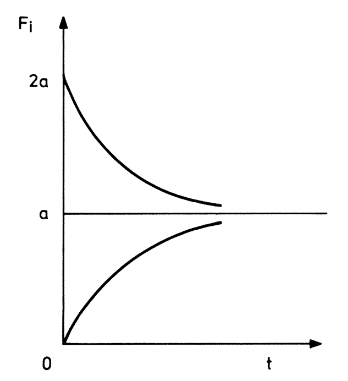
\includegraphics[width=0.95\textwidth]{img/Figura5-11.png}
    \end{minipage}%
    % --- COLUMNA DERECHA (Fórmulas) ---
    \begin{minipage}{0.45\textwidth}
        \vspace{1.5cm} 
        \begin{align*}
            F_1(t) &= a(1+e^{-kt}) \\
            F_2(t) &= a \\
            F_3(t) &= a(1-e^{-kt}) \\[1em]
            \text{con } & a, k \in R^+.
        \end{align*}
    \end{minipage}

    \vspace{10pt} % Un pequeño espacio vertical entre la imagen/fórmulas y el texto
    
    
    \parbox{\textwidth}{
        \centering
        \scriptsize 
        \text{Fig. 5.11.} Tres formas diferentes de alcanzar el mismo estado final o valor asintótico
        
        $X_{\infty} = a$ partiendo de $a$, avanzando hacia él o declinando hacia él.
    }
    
    \end{figure}

    \subsection*{(d)\textit{ Memoria}}
    \noindent Supongamos que el estado de una cosa depende no solo de un parámetro $t$ (la fase
    del proceso), sino también de algún estado o estados anteriores. 
    En este caso, se dice que la cosa tiene {\textit{memoria}} de algunos de sus estados pasados, 
    o que sufre un proceso {\textit{hereditario}}. Así, el estado elástico de una pieza
    de acero, el estado magnético de un imán y el estado genético de un organismo 
    dependen todos de sus historias previas. En varios casos, esa dependencia puede expresarse mediante una fórmula del tipo

    \[
        F(t) = \int_0^t F(\tau - t) \cdot M(\tau) \cdot \mathrm{d}\tau,
    \]

    \noindent donde $M$ es la función de memoria. (El proceso no tiene memoria si es $M$ = $\delta$,
    o la delta de Dirac).

    El concepto general se aclara mediante

    \medskip

    \noindent DEFINICIÓN 5.20 Sea $\mathbb{F}$ una función de estado y $S(x)$ el espacio de estados correspondiente,
    para una cosa $x$ relativa a un cierto marco de referencia. Además,
    llámese a $t \in T$ el parámetro de estado, donde $T$ es un conjunto dirigido. 
    Entonces $x$ experimenta un proceso {\textit{hereditario}} si y solo si cada uno de sus estados $\mathbb{F}(t) \in S(x)$ es un funcional 
    de algunos otros estados $\mathbb{F}(\tau)$ con $\tau<(t)$.

    Hay dos tipos importantes de procesos hereditarios: ($a$) la
    memoria se mantiene bastante intacta durante todo el proceso, y ($b$ ) 
    la memoria se desvanece hasta desaparecer prácticamente después de un cierto tiempo llamado {\textit{tiempo de relajación}}. 
    Los sistemas con componentes que interactúan débilmente, como
    los gases no ionizados y los imperios extendidos, tienen tiempos de relajación cortos. 
    Por otro lado, los organismos tienen tiempos de relajación genética y ontogenética largos. 
    Por ejemplo, la desnutrición y la privación de la socialidad en las primeras etapas de la vida de un mamífero son suficientes 
    por separado para perjudicar gravemente algunas de sus capacidades para la vida.

    \subsection*{(e)\textit{ Reversibilidad e irreversibilidad}}
    \noindent Algunos procesos, especialmente a nivel microfísico —y probablemente solo esos—, son reversibles; todos los macroprocesos conocidos son irreversibles.
    Esto último puede considerarse una generalización de un teorema demostrado en mecánica estadística. Un sistema se denomina {\textit{érgodico}} si finalmente explora todo su espacio de estados o, 
    más precisamente, si, cuando se deja inalterado (aislado), ocupa sucesivamente todos los estados compatibles con su energía total.

    \smallskip

    \noindent Hasta 1913, la mayoría de los autores afirmaban que, dado que las partículas individuales se mueven
    de forma reversible, toda colección de partículas debe tener la propiedad de reversibilidad y, además, debe ser ergódica. 
    Ese año, A. Rosenthal y M. Plancherel demostraron de forma independiente que, si el sistema satisface las ecuaciones canónicas (cap. 3, sec. 2.6), entonces no es ergódico. 
    Es decir, demostraron que no existen sistemas ergódicos (o totalmente reversibles) de la mecánica clásica. 
    Por lo tanto, incluso si el universo fuera un enorme agregado de partículas (que no lo es), no podría volver sobre todos sus pasos. 
    No existe el eterno retorno.

    Finalmente, observamos que en microfísica se asume que la mayoría de los procesos, aunque no todos, son {\textit{estocásticamente reversibles}}, 
    en el sentido de que la probabilidad de un proceso elemental y la de su inverso son iguales. Esto permite desviaciones momentáneas de la tendencia general, 
    es decir, eventos aislados en los que algunos estados se vuelven superpoblados o subpoblados. Sin embargo, ciertos microprocesos, en particular la radiactividad y, 
    en general, los procesos de transmutación, son irreversibles.

    Todo esto invita a

    \smallskip

    \noindent DEFINICIÓN 5.21 Sea $\pi(x) = \langle \mathbb{F}(t) \mid t \in T \rangle$ En un proceso serial en una cosa x.
    Además, sea $\bar{T}$ el mismo conjunto que $T$ dirigido en sentido opuesto (por ejemplo, $\langle \mathbb{R}, > \rangle$  en lugar de $\langle \mathbb{R}, < \rangle$. 
    Entonces $\pi(x)$ es reversible si y solo si $\bar{\pi}(x) = \langle \mathbb{F}(t) \mid t \in \bar{T} \rangle$ es tan posible (es decir, legal) como $\pi(x)$.

    Si tanto a $\pi(x)$ como a su inverso $\bar{\pi}(x)$ se les pueden asignar 
    probabilidades, se puede pensar en definir el \textit{grado de reversibilidad} 
    de un proceso como la razón de su probabilidad y la de su inverso, o 
    $r = \bar{p}/p$. Para un proceso totalmente reversible, $r=1$; para un 
    proceso bastante reversible, $0 \ll r < 1$; para un proceso casi irreversible, 
    $0 < r \ll 1$; y para un proceso totalmente irreversible, $r=0$. 
    Tal concepto podría ser útil en varios campos, particularmente en la 
    mecánica estadística.

    Es común declarar que un proceso es reversible solo en caso de que sus leyes 
    sean invariantes bajo la inversión del tiempo. Esto es un error, porque los 
    procesos dependen tanto de las circunstancias como de las leyes. Por ejemplo, 
    aunque las leyes básicas de la desintegración radioactiva (principalmente 
    las de Schrödinger) son $T$-invariantes, las condiciones de frontera son tales 
    que la probabilidad de que un fragmento de la desintegración reingrese al 
    núcleo se anula.

    Finalmente, nótese que, si bien todos los procesos reversibles son cíclicos, 
    lo contrario es falso. De hecho, la mayoría de los ciclos no son reversibles – 
    es decir, no dejan las cosas como estaban. Por ejemplo, el ciclo del agua y el 
    ciclo del nitrógeno en nuestro planeta no son reversibles, ya que están 
    acompañados por una degradación de la energía (aumento de la entropía).

    \subsection*{(f)\textit{ Proceso aleatorio}}
    \noindent Un tipo conspicuo de proceso en serie, y uno de gran interés filosófico, 
    es el de un proceso aleatorio. (Para una definición de aleatoriedad, 
    véase Cap. 4, Sec. 6.4.) Un proceso aleatorio o estocástico es aquel 
    que se describe por una función de estado que es una “variable” aleatoria, 
    es decir, una función cada uno de cuyos valores tiene una probabilidad 
    o densidad de probabilidad definida. En el caso más simple, los valores 
    $s_i$ de la función de estado $\mathbb{F}$ forman una secuencia discreta 
    $\langle s_i \mid i \in \mathbb{N} \rangle$, como los tiempos de llegada de 
    los clientes a un mostrador. En este caso, la función $f$ tal que 
    $f(s_i) = \mathrm{Pr}(\mathbb{F}(t) = s_i) = p_i$, donde $\mathrm{Pr}$ 
    es una medida de probabilidad y $p_i$ la probabilidad de que $x$ se encuentre 
    en el estado $s_i$, se denomina la \textit{distribución de probabilidad} 
    de $\mathbb{F}$. (Véase, por ejemplo, Feller, 1968, Cap. IX.)

    Muchas propiedades sustanciales, en todos los niveles, deben ser representadas 
    por ``variables'' aleatorias. Por lo tanto, cualquier proceso real ---en 
    contraste con un modelo idealizado del mismo--- es probable que tenga al menos 
    un aspecto aleatorio. Por consiguiente, en lugar de definir el concepto de 
    un proceso real (como es habitual en la bibliografía sobre procesos 
    estocásticos) preferimos adoptar


    \noindent DEFINICIÓN 5.22 Sea $\mathbb{F}$ $ = \langle F_1, F_2, \dots, F_n \rangle$ 
    una función de estado para una cosa $x$ que experimenta un cambio en serie 
    $\pi(x) = \langle \mathbb F(t) \mid t \in T \rangle$. Se dice que este proceso es 
    \textit{aleatorio en el i-ésimo aspecto} si y solo si la componente $F_i$ 
    de $\mathbb{F}$ es una variable aleatoria.

    \subsection*{(g)\textit{ Estabilidad}}
    \noindent Se dice que una cosa es estable si su punto representativo en el espacio de 
    estados permanece confinado dentro de una región ``pequeña''. Más 
    precisamente, podemos hacer

    \bigskip

    \noindent DEFINICIÓN 5.23 Sea $G_{\mathbb{L}}(x)$ el conjunto de transformaciones 
    lícitas del espacio de estados $S_{\mathbb{L}}(x)$ de una cosa $x$. Entonces $x$ es 
    \textit{estable en la región} $A \subset S_{\mathbb{L}}(x)$ si y solo si, para todo 
    $s \in S_{\mathbb{L}}(x)$, $g(s) \in A$ para todo $g$ en $G_{\mathbb{L}}(x)$.

    En otras palabras, una cosa está en un estado de \textit{equilibrio dinámico} 
    si todos los cambios que experimenta la llevan a un subconjunto fijo de su 
    espacio de estados. Si este subconjunto se reduce a un punto, entonces se 
    dice que la cosa está en \textit{equilibrio estático} o que no cambia en 
    absoluto. En otras palabras, una cosa $x$ está en equilibrio estático en un 
    estado $a \in S_{\mathbb{L}}(x)$ si y solo si $a$ es un punto fijo bajo cada 
    transformación del espacio de estados en sí mismo ---es decir, si $g(a) = a$ 
    para todo $g \in G_{\mathbb{L}}(x)$. En resumen, así como los subconjuntos fijos 
    del espacio de estados representan el equilibrio dinámico, los puntos fijos 
    representan los estados de equilibrio estático.

    Los estados de equilibrio estático solo pueden ser temporales. Por otro lado,
    el equilibrio dinámico puede ser duradero. La figura 5.12 muestra los estados de

    \newpage

    \begin{center}
        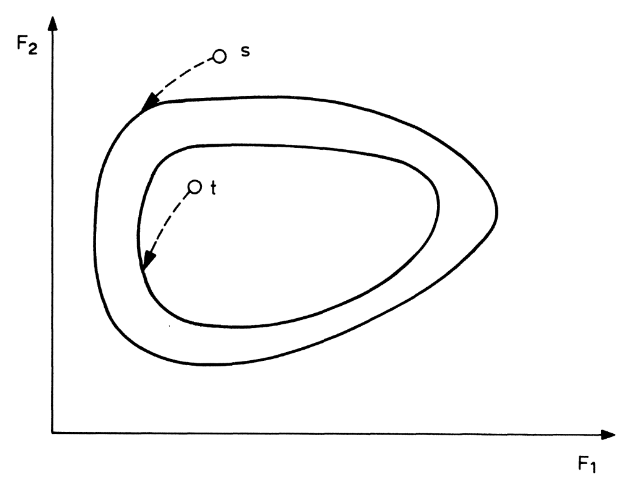
\includegraphics[width=0.8\textwidth]{img/Figura5-12.png}
        \\ \scriptsize Fig. 5.l2. Los equilibrios ecológicos son dinámicos. 
            Si una perturbación externa, como la agricultura o una sequía, envía el 
            punto representativo a $s$, o a $t$, el punto finalmente se mueve a una 
            órbita de equilibrio. (Véase, por ejemplo, Pielou (1969).)
    \end{center}

    \noindent equilibrio dinámico de un ecosistema que consiste en dos poblaciones en 
    competencia. Cada curva representa un proceso cíclico ---una oscilación 
    en el número de las poblaciones. Cada punto situado sobre una de las 
    curvas cerradas representa un estado estable del sistema. Si las poblaciones 
    son desplazadas ---por ejemplo, por alguna perturbación externa--- a valores 
    no muy lejanos del equilibrio, tienden a regresar espontáneamente a un 
    punto de equilibrio.

    Hasta aquí los tipos especiales de procesos. Apresurémonos a advertir que, 
    en nuestra opinión, ningún proceso real es de un tipo puro. Esto se debe a 
    que cualquier función de estado (realista) tiene una serie de componentes 
    de diferentes tipos ---algunos discretos, otros continuos, algunos aleatorios, 
    otros no aleatorios, y así sucesivamente. En otras palabras, llámese

    \[
        \pi_k(x) = \langle F_k(t) \mid t \in T \rangle, \quad \text{con } 1 < k \leq n
    \]

    \noindent la \textit{k-ésima componente} del proceso en serie representado por 
    $\pi(x)$ =$\langle \mathbb{F}(t) \mid t \in T \rangle$. Entonces $\pi(x)$ tendrá 
    al menos una componente continua, al menos una componente aleatoria, y así 
    sucesivamente. En resumen, los tipos de procesos puros

    \newpage

    \noindent son tipos ideales: los procesos reales son impuros. Dejamos la formulación
    exacta para la siguiente subsección.

    En primer lugar, nos centraremos en algunas generalidades que pueden formularse en términos bastante
    exactos.

    \subsection{Conceptos y principios generales}
    \noindent En la subsección anterior discutimos algunos tipos de procesos típicos. 
    En la presente trataremos los procesos en general, utilizando algunas ideas 
    obtenidas en el estudio de tipos de procesos especiales. De ese estudio se 
    desprende que un proceso puede ser considerado ya sea como una \textit{secuencia 
    de estados} o como una \textit{secuencia de eventos}. En el primer caso podemos 
    describir un proceso en una cosa $x$ con la única ayuda de una función de estado 
    $\mathbb{F}$ para ello: nuestra tarea se reduce a seguir los recorridos de la 
    punta de $\mathbb{F}$ ---una tarea enormemente facilitada al parametrizar los 
    estados $\mathbb{F}(t)$ en relación con los estados de un marco adecuado. Si, 
    por otro lado, interpretamos un proceso como una secuencia de eventos, entonces 
    se nos debe dar no solo $\mathbb{F}$ sino también todo el espacio de estados 
    $S_{\mathbb{L}}(x)$ abarcado por $\mathbb{F}$, así como la totalidad $G_{\mathbb{L}}(x)$ de 
    las transformaciones lícitas del espacio de estados en sí mismo. Solo esto 
    nos permite formar los eventos individuales $\langle s, s', g \rangle$ y, a 
    partir de ahí, todo el espacio de eventos $E_{\mathbb{L}}(x)$.

    Cada una de estas interpretaciones alternativas tiene sus ventajas y desventajas. 
    El enfoque de los estados sucesivos es matemáticamente más simple, aunque solo 
    sea porque el espacio de estados es $n$-dimensional mientras que el espacio 
    de eventos correspondiente es $2n$-dimensional. Por otro lado, el enfoque 
    de los eventos sucesivos, aunque matemáticamente más torpe, es filosóficamente 
    más perspicaz. Podemos usar cualquiera de los dos enfoques indistintamente y 
    así lo haremos. En la presente subsección discutiremos algunos principios 
    generales en términos de eventos, pero terminaremos introduciendo una noción 
    de historia basada en el enfoque de los estados sucesivos.

    Primero, las nociones generales del proceso:

    \bigskip

    \noindent DEFINICIÓN 5.24 Sea $E_g(x)$ el espacio de eventos de tipo 
    $g$ en la cosa $x$, para $g$ en el conjunto $G_{\mathbb{L}}(x)$ de transformaciones 
    lícitas del espacio de estados escogido para $x$, y sea $E(x)$ la unión de 
    todos los $E_g(x)$'s, es decir, el espacio total de eventos de $x$ 
    [Definición 5.9]. Además, sea $<$ la relación de precedencia [Definición 5.10]. 
    Entonces 
    
    (i) un \textit{proceso de tipo g} en la cosa $x$ es un conjunto 
    estrictamente parcialmente ordenado de eventos de clase $g$:

    \[
        \pi_g(x) = \langle E_g^*(x), < \rangle \quad \text{con } E_g^*(x) 
        \subseteq E_g(x) \subseteq E_\mathbb{L}(x);
    \]

    (ii) un proceso en x es un conjunto estrictamente parcialmente ordenado

    \[
        \pi(x) = \langle E^*(x), < \rangle \quad \text{con} \quad E^*(x) = 
        \bigcup_{g \in G_\mathbb{L}(x)} E_g^*(x).
    \]

    Dado que, de hecho, cada aspecto g está relacionado con algún otro aspecto,
    podemos suponer con seguridad que no hay procesos de un solo tipo, sino
    solo idealizaciones que destacan ahora una característica de lo que nos interesa,
    ahora otra. (Recuerde el final de la última subsección). Es decir, suponemos

    \bigskip

    \noindent POSTULADO 5.6 Todo proceso real tiene más de un aspecto.

    Y de la supuesta legalidad de las transformaciones en $G_{\mathbb{L}}(x)$se deduce
    que todo proceso que implique una cosa determinada satisface todas las leyes
    que posee esta última:

    \bigskip

    \noindent COROLARIO 5.9 Todos los procesos son legales.

    Tenga en cuenta que la legalidad se basa en procesos, es decir, en conjuntos de eventos intrínsecamente ordenados,
    y no en conjuntos de eventos arbitrarios. Estos últimos, especialmente si ocurren en cosas no relacionadas, o en cosas 
    con componentes débilmente acoplados,
    no son necesariamente legales, aunque se suponga que cada componente tiene una línea de comportamiento legal.
    Esto es el Este es el fundamento ontológico de la regla metodológica empleada tácitamente por
    los historiadores que se proponen descubrir tendencias históricas generales o incluso leyes,
    es decir, centrarse en procesos de un tipo definido que se producen en los sistemas sociales
    en lugar de limitarse a buscar series temporales, que están destinadas a ser
    erráticas o ilegales (véase Braudel, 1969).

    Recuerde, sin embargo, que el caos no es lo mismo que la aleatoriedad: mientras que el primero carece de ley, 
    el segundo posee leyes estocásticas (probabilísticas) como las de la mecánica cuántica y la genética. Por lo tanto, 
    adoptamos un axioma que emplea la Definición 5.22 de un proceso aleatorio en algún aspecto:
    
    \bigskip

    \noindent POSTULADO 5.7 Todo proceso es aleatorio en al menos un aspecto.

    Luego distinguimos dos miembros importantes de un proceso:

    \bigskip

    \noindent DEFINICIÓN 5.25 Sea $\pi(x) = \langle E^*(x), < \rangle$ 
    un proceso en una cosa $x$. Entonces

    (i) $\pi(x)$ \textit{comienza} en un evento $b \in E^*(x)$ si y solo 
    si $b$ es una cota inferior del conjunto $E^*(x)$ [es decir, si cualquier 
    otro miembro de $E^*(x)$ sigue a $b$];

    (ii) $\pi(x)$ \textit{termina} en un evento $e \in E^*(x)$ si y solo 
    si $e$ es una cota superior del conjunto $E^*(x)$ [es decir, si todos los 
    demás miembros de $E^*(x)$ preceden a $e$].

    \begin{center}
        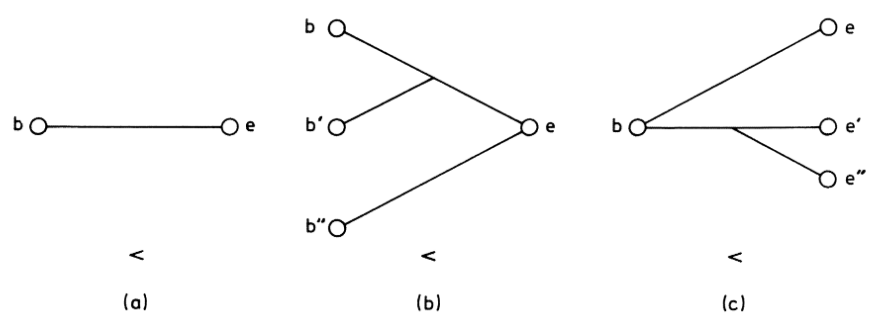
\includegraphics[width=0.8\textwidth]{img/Figura5-13.png}
        \\ \scriptsize Fig. 5.l3. Tres tipos de procesos en cuanto al inicio y el final. (a) Proceso en cadena o lineal. (b)
        Proceso convergente o ramificado. (c) Proceso divergente o ramificado.
    \end{center}

    Un proceso puede no tener un único inicio ni un único final: véase la figura 5.13.
    En otras palabras, puede haber múltiples inicios o múltiples finales. Suponemos 
    que cada proceso está limitado tanto por arriba como por abajo:

    \bigskip

    \noindent POSTULADO 5.8 Todo proceso tiene principio(s) y fin(es). 
    [Es decir, si $\pi(x)$ es un proceso que ocurre en una cosa $x$, entonces 
    $\pi(x)$ tiene al menos un principiante y al menos un punto final.]

    Esta hipótesis no implica que haya comienzos absolutos (es decir, procesos 
    que empiezan de la nada) y callejones sin salida (es decir, procesos que, 
    al terminar, no inician ningún otro proceso). De hecho, el postulado es compatible 
    tanto con una cosmología creacionista y escatológica como con la suposición de que 
    cada proceso en una cosa dada, aunque limitado tanto por abajo como por arriba, 
    está precedido y seguido por otros procesos, ya sea en la misma cosa o en otras cosas. 
    Adoptamos la última hipótesis porque es la que respalda la ciencia. Pero primero necesitamos

    \bigskip

    \noindent DEFINICIÓN 5.26 Sean $\pi(x)=\langle E^*(x), < \rangle$ y 
    $\pi'(x)=\langle E'^*(x), < \rangle$ dos procesos en una cosa $x$, tales que 
    $E^*(x) \cap E'^*(x) = \emptyset$. Entonces $\pi(x)$ \textit{precede} a 
    $\pi'(x)$ si y solo si cada evento en el primero precede a cada evento en el 
    segundo. Símbolo: $\pi(x) < \pi'(x)$.

    Estamos listos para

    \bigskip

    \noindent POSTULADO 5.9 Cada proceso está precedido y seguido por otros procesos. 
    Más precisamente, cada cosa $x$ tiene partes $y$ y $z$, no necesariamente diferentes de $x$, 
    cada una de ellas equipada con su propio espacio de eventos, de tal manera que.

    \[
        \pi(y) < \pi'(x) < \pi''(z).
    \]

    Dado que el mundo es la suma de todas las cosas, se deduce que

    \bigskip

    \noindent COROLARIO 5.10 El mundo no tiene principio ni fin.

    \textit{Observación 1} Al igual que muchos otros axiomas de nuestra ontología, el anterior
    es una especie de generalización de todo lo que sabemos. Un paradigma antiguo es,
    por supuesto, el proceso de nacimiento-crecimiento-desintegración final que experimenta todo metazoario. 
    Un paradigma más simple y moderno es el del fotón emitido por una estrella, que viaja a través del espacio interestelar y termina
    atrapado por una molécula o convirtiéndose en un par de electrones de cargas opuestas.
    \textit{Observación 2} En un momento dado, algunos cosmólogos que deseaban salvar la cosmología del estado 
    estacionario introdujeron la hipótesis \textit{ad hoc} de la creación espontánea de átomos de hidrógeno en el espacio vacío. 
    Esta conjetura no fue aceptada porque choca con las leyes de conservación (Bunge, 1962) y, en cualquier caso, 
    la teoría del estado estacionario, que intentaba salvar, fue finalmente refutada por las pruebas astronómicas.
    \textit{Observación 3} Corolario 5.10 Fue formulado por primera vez por los filósofos presocráticos y adoptado por Aristóteles. 
    Parecería contradecir la hipótesis del ``Big Bang'' sobre el ``origen'' del universo, hoy en día casi universalmente aceptada. 
    Sin embargo, esta conjetura cosmológica —que explica la expansión del universo— no ilustra la creación \textit{ex nihilo}, ya que presupone que
    el universo existía —en un estado altamente condensado— antes de que comenzara la expansión. Tampoco la antigua hipótesis 
    de la ``muerte térmica'' (hoy en día casi olvidada) ilustra la aniquilación absoluta: lo único que afirma es el fin del movimiento macrofísico 
    una vez que un sistema cerrado ha alcanzado el equilibrio térmico.

    Hasta aquí nuestros conceptos y principios generales sobre el proceso. Adoptemos ahora el enfoque de los estados sucesivos e introduzcamos una 
    noción clave más que resultará indispensable en la secuela, a saber, la de historia.

    Recuérdese que los estados de una cosa $x$ pueden ser coordenados en relación 
    con los estados $t \in S(f)$ de un marco de referencia $f$, definiendo la 
    función de estado como una aplicación de $S(f)$ en $S(x)$, y construyendo 
    $S(f)$ como una cuadrícula cuatridimensional que conceptualiza un marco de 
    referencia físico (Sec. 2.5). A medida que el estado de referencia $t$ se 
    ``mueve'', también lo hace la punta $\mathbb{F}(t)$ de la función de estado de la cosa. 
    Esto invita

    \bigskip

    \noindent DEFINICIÓN 5.27 Sea $\mathbb{F}$ una función de estado para 
    una cosa $x$ relativa a un marco de referencia $f$ con estados $t \in S(f)$, 
    y sea este último coordenado por una cierta función $k: \mathbb{R}^4 \to S(f)$. 
    Entonces la \textit{historia de $x$ relativa a $f$} es el conjunto de pares 
    ordenados

    \[
        h(x) = \{\langle t, \mathbb{F}(t) \rangle \mid t \in S(f)\}.
    \]

    Esta es una elucidación del concepto de línea de vida, línea de comportamiento 
    o trayectoria. La historia de una cosa se considera como la sucesión de sus 
    estados pero, en lugar de ser representada por una línea en el espacio de 
    estados $n$-dimensional abarcado por $\mathbb{F}$, se representa como una 
    curva en el espacio ($n+4$)-dimensional $\mathbb{R}^4 \times S_\mathbb{L}(x)$. 
    (La dimensionalidad de este espacio puede reducirse en 3 si estamos interesados 
    solo en la coordenada temporal, es decir, si $t$ se interpreta como un instante 
    de tiempo en lugar de como un punto en la región del espaciotiempo adjunta al 
    marco dado.)

    La definición anterior abarca los conceptos más habituales de historia empleados 
    en las ciencias. En particular, encaja con el concepto de historia que aparece en 
    una de las teorías más fundamentales de la física, a saber, la mecánica cuántica. 
    De hecho, en esta teoría, el operador de evolución de una cosa se define como

    \[
        S(t_0, t) = \exp\left(-\frac{i}{\hbar}\int_{t_0}^{t} du H\right),
    \]

    \newpage

    \noindent donde H es el hamiltoniano de la cosa. La historia de este último es entonces
    \[
        h(x) = \{\langle \langle t, S(t_0, t) \rangle \psi(t_0) \rangle \mid u \in [t_0, t] \ \& \ \psi \in \text{espacio de Hilbert de } x\}.
    \]

    El amplio concepto de historia adoptado anteriormente puede desconcertar e 
    incluso enfurecer a aquellos estudiosos de las humanidades que todavía 
    consideran al hombre como algo sobrenatural. Hasta aproximadamente mediados 
    del siglo XIX se había asumido tácitamente que toda la historia es historia 
    humana. Así, Hegel, a pesar de todo su dinamismo, negaba que la naturaleza 
    tuviera una historia. Esa visión cambió con los descubrimientos revolucionarios 
    en geología y biología, hasta el punto de que Engels declaró que cada ciencia 
    es la historia de algo (Engels, 1878). Desde entonces, se suele dar por sentado 
    que \textit{toda cosa tiene una historia} ---es decir, que, para toda cosa $x$, 
    $h(x)$ es más grande que un singulete.

    Apliquemos ahora el concepto de historia a una caracterización de las nociones 
    de acción e interacción.

    \bigskip

    \section{\centering ACCIÓN Y REACCIÓN}

    \subsection{Cambio inducido}
    Hasta ahora nos hemos ocupado del cambio sin tener en cuenta sus
    orígenes. Ahora bien, una cosa puede cambiar por sí misma o bajo la influencia
    de otra cosa, es decir, espontáneamente o por inducción. Por lo tanto, debemos
    estudiar los conceptos de espontaneidad e inducción. Para ello,
    nos valeremos del concepto de historia (Definición 5.27 en la Sec.
    3.2) y de la ley de Leibniz (Cap. 2, Sec. 3.2).
    Dos cosas diferentes del mismo tipo pueden describirse con la ayuda
    del mismo esquema funcional (M, IF), por lo tanto, del mismo espacio de estados,
    aunque, por supuesto, añadiendo circunstancias individualizadoras en cada caso. En
    otras palabras, los estados de cosas diferentes del mismo tipo pueden representarse en
    un mismo espacio de estados. Además, cada espacio de estados, lejos de ser
    propiedad de una sola cosa, puede asignarse a una clase de referencia constituida por
    una clase de equivalencia más o menos numerosa de cosas. Ahora bien, la ley de Leibniz
    (Postulado 2.5 o Corolario 2.1) establece que cosas diferentes tienen propiedades diferentes.
    Por lo tanto, incluso si una función de estado dada describe adecuadamente
    dos cosas, estas no pueden ocupar exactamente los mismos estados, ya que, si lo hicieran,
    serían una sola. En consecuencia, tenemos la siguiente reformulación de
    la ley de Leibniz: 

    COROLARIO 5.11 Las cosas diferentes tienen historias diferentes.
    Sin duda, una cosa puede ocupar ahora exactamente el mismo estado en el que se encontraba otra cosa
    hace un momento, pero no hay dos cosas que puedan ocupar exactamente el mismo
    estado al mismo tiempo o, más en general, para el mismo valor del
    parámetro de cambio. (Véase la figura 5.14). 

    \begin{figure}[h!]
    \centering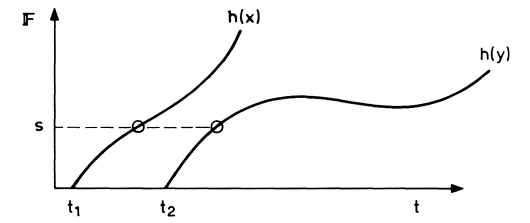
\includegraphics[width=0.6\textwidth]{img/grafico5.14.png}
    \caption{\label{fig:espacio_estados} Fig. 5.14. Diferentes cosas pueden ocupar el mismo estado siempre que lo hagan en
    momentos diferentes.}
    \end{figure}

    \begin{center}
        CAMBIO
    \end{center}

    El corolario 5.11 es nuestra versión actual del principio de
    individuationis de Leibniz y nos da la clave de lo que buscamos. De hecho, si una
    cosa está bajo la acción de otra cosa, entonces su historia debe diferir
    de la historia cuando está libre de dicha acción. (Véase la figura 5.15). (En esto
    consiste el experimento científico, a diferencia de la observación,
    es decir, en activar y desactivar deliberadamente acciones o influencias para
    comparar el comportamiento forzado de una cosa con su comportamiento libre y así
    evaluar la importancia de la variable que se está manipulando).

    \begin{figure}[h!]
    \centering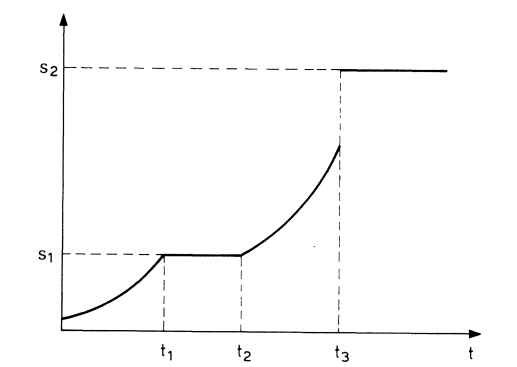
\includegraphics[width=0.6\textwidth]{img/grafico5.15.png}
    \caption{\label{fig:grafico_5_15} Fig. 5.15. [Fig. 5.15. Ejemplo imaginario de una acción. El agente, al actuar durante el intervalo [f1, t2],
    obliga al paciente a permanecer en el estado 51'. La acción externa se reanuda en el momento f3,
    obligando al paciente a saltar al estado 52'. ].}
    \end{figure}

    En ausencia de cualquier acción del agente x sobre el paciente y, la
    historia de su suma física o yuxtaposición x + y es igual a la unión de
    sus líneas de comportamiento individuales. En otras palabras, tenemos

    DEFINICIÓN 5.28 La cosa x cambia por sí misma, o espontáneamente, si y solo si h(x) no es
    un singleton y, para cualquier otra cosa y

    \begin{center}
        $h(x \dot{+} y) = h(x) \cup h(y)$.
    \end{center}
    
    Claramente, si una de las cosas actúa sobre la otra, entonces, mientras que la
    línea de comportamiento del agente permanece inalterada, la del paciente

    \begin{center}
        CAPÍTULO 5
    \end{center}

    se convierte, por así decirlo, en la historia de otra cosa a saber,
    la cosa sobre la que actúa el agente. (Véase la figura 5.16.) Más exactamente, hacemos

    \begin{figure}[h!]
    \centering
    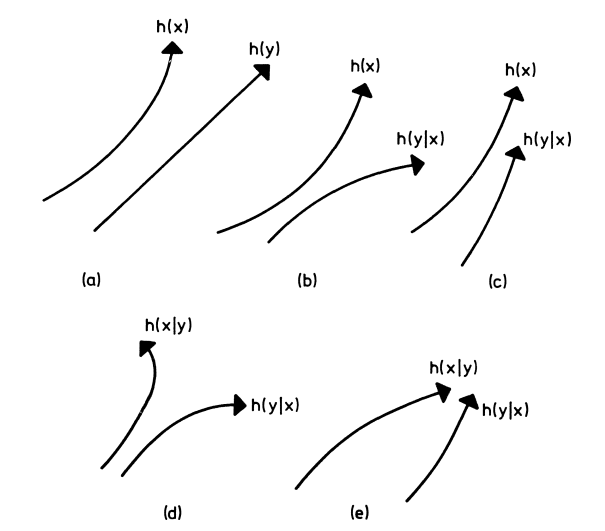
\includegraphics[width=0.6\textwidth]{img/grafico5.16.png}
    \caption{\label{fig:grafico_5_16} Fig. 5.16. [Cambio inducido. (a) Sin acción: cambio espontáneo tanto de x como de y.
    (b) Acción de empuje de x sobre y. (c) Acción de tracción de x sobre y. (d) Interacción de empuje.
    (e) Interacción de tracción. ].}
    \end{figure}

    DEFINICIÓN 5.29 Sean X e y dos cosas diferentes con funciones de estado IF y G respectivamente relativas a un marco de referencia común t, y 
    sea
    
    \begin{center}
        $$ h(y|x) = \{ \langle t, \mathbb{H}(t) \rangle | t \in S(f) \} $$
    \end{center}

    serán sus respectivas historias. Además, sea IHI = g(lF, G) ¢ G una tercera función de estado,
    dependiente tanto de IF como de G, y llamemos

    \begin{center}
        $$ h(x) = \{ \langle t, F(t) \rangle | t \in S(f) \}, \quad h(y) = \{ \langle t, G(t) \rangle | t \in S(f) \} $$
    \end{center}

    La historia correspondiente. Entonces x actúa sobre y, o x [> y para abreviar, si y solo si, para
    alguna función de estado IHI que determina la trayectoria h (y Ix),
    h (y Ix) ¢ h (y ).

    \bigskip

    \begin{center}
        CAMBIO
    \end{center}

    Ahora podemos reformular la definición 5.28 de espontaneidad: Una cosa
    cambia espontáneamente si y solo si cambia y no hay ninguna otra cosa que
    actúe sobre ella. Y, a partir de la hipótesis de la definición 5.29 (en particular,
    que x '¢ y), se deduce que nada actúa sobre sí mismo.
    La definición de acción recíproca o mutua es ahora obvia:

    DEFINICIÓN 5.30 Dos cosas diferentes x e y interactúan si y solo si cada una actúa sobre
    la otra. En símbolos:

    \begin{center}
        $$ x \bowtie y =_{\text{df}} x \rhd y \ \& \ y \rhd x. $$
    \end{center}

    Los científicos experimentales asumen tácitamente (a) que todas las cosas son estudiables,
    (b) que no hay cosas totalmente aisladas, es decir, que cada cosa actúa sobre otra cosa
    o es afectada por otra cosa, y (c) que tales acciones son la base
    del conocimiento empírico. De hecho, si una cosa supuesta no actúa sobre ninguno
    de nuestros medios de observación, entonces no podemos observarla; y si alguna
    cosa putativa no es afectada por ninguno de nuestros medios experimentales, entonces
    no podemos experimentar con ella. En cualquiera de los dos casos, no nos preocuparemos por «ella». En
    resumen, el siguiente axioma pertenece a la ontología inherente a la ciencia,
    por lo que lo adoptamos:

    POSTULADO 5.10 Todo actúa sobre otras cosas y es afectado por ellas.
    Esta suposición no debe confundirse con la hipótesis mucho más fuerte y
    Esta suposición no debe confundirse con la hipótesis mucho más fuerte, y
    falsa, de que dos cosas cualesquiera interactúan, y mucho menos con la misma
    intensidad. No reaccionamos ante la actividad luminosa del sol, y mucho menos
    ante la de una estrella extinta. En otras palabras, el principio de interacción universal,
    sugerido por primera vez por los estoicos y muy favorecido durante el
    apogeo de la teoría de la gravitación de Newton, es falso.
    Los efectos de una interacción pueden ser duraderos, incluso en el caso de
    las microcosas. Así, si dos microcosas interactúan durante un tiempo y luego dejan
    de hacerlo, por ejemplo, al separarse mucho en el espacio, seguirán
    estando correlacionadas. Por lo tanto, observar una de ellas puede proporcionar
    información sobre la otra, del mismo modo que observar el comportamiento de una
    persona divorciada puede arrojar luz sobre su antigua pareja. En la jerga de la
    mecánica cuántica, se dice que tales cosas son inseparables o que
    muestran una correlación EPR. (Esto es lo que parece ser la paradoja de Einstein-Podolsky-Rosen.
    Más información en la sección 4.2).

    \bigskip

    Necesitamos un concepto cualitativo del tamaño de una acción o una interacción. Este viene dado por la cantidad de distorsión efectuada por el
    agente o agentes en la línea de comportamiento del paciente. En otras palabras, hacemos
    
    DEFINICIÓN 5.31 Sean x e y dos cosas, y sea h(x) la historia
    de x, y h(xl y) la historia de x cuando actúa sobre y, y de manera similar para
    x. Entonces
    (i) la acción o efecto total de x sobre y es igual a la diferencia entre
    la trayectoria forzada y la trayectoria libre de y:

    \begin{center}
        $$ A(x, y) = h(y|x) \cap \overline{h(y)}; $$
    \end{center}

    (ii) la reacción total de y sobre x es la diferencia entre la trayectoria libre
    y la trayectoria forzada de x:

    \begin{center}
        $$ A(y, x) = h(x|y) \cap \overline{h(x)}; $$
    \end{center}

    (iii) la interacción total entre x e y es la unión de acción y
    reacción:

    \begin{center}
        $$ I(x, y) = A(x, y) \cup A(y, x). $$
    \end{center}

    Si A (x, y) = 0, podemos decir que x ejerce una acción nula sobre y.
    Dado que la acción de x sobre y es un conjunto de eventos en y, este conjunto no puede ser el
    mismo que la reacción de y sobre x, que es un conjunto de eventos en x. Por lo tanto, tenemos
    el

    \noindent COROLARIO 5.12 Ninguna acción es igual a la reacción correspondiente. Es decir, para
    cualquier cosa x e y, A(x, y):I= A(y, x).
    Este resultado no es inconsistente con la tercera ley de la mecánica de partículas newtoniana.
    De hecho, esta ley no afirma que las acciones y reacciones sean
    iguales, sino que sus intensidades (las fuerzas correspondientes, o bien
    los pares) son iguales. De todos modos, la ley no se cumple en otras teorías, como
    la electrodinámica.

    Ahora bien, las acciones pueden existir en ciertos aspectos, pero no en otros. Es decir,
    la acción de la cosa x sobre la cosa y puede afectar solo a algunos de los
    componentes de la función de estado de y. Por lo tanto, podemos analizar la acción total
    en acciones parciales, a saber: 

    \begin{center}
        $$ A(x, y) = \bigcup_{i=1}^{m} A_{i}(x, y), $$
    \end{center}

    \smallskip

    \begin{center}
        CAMBIO
    \end{center}

    Donde m es el número de acciones mutuamente independientes que x ejerce sobre
    y. Lo mismo ocurre con la reacción de y sobre x y con su interacción.
    Esta distinción nos permite complementar el Postulado 5.8 con

    POSTULADO 1E 5.11 Todo cambia espontáneamente en algunos aspectos,
    y de forma inductiva en otros.
    Por último, el concepto de acción nos permite dilucidar la importante
    distinción que se hace en el capítulo 2, sección 5.1, entre una relación que afecta a sus
    relata y otra que no lo hace. (Véase la figura 5.17.) La diferencia se
    precisa mediante

    DEFINICIÓN 5.32 Dos cosas diferentes están unidas (o vinculadas o
    acopladas) entre sí si y solo si al menos una de ellas actúa sobre la otra. En
    símbolos: si x e y son cosas, entonces

    \begin{center}
        $$ Bxy =_{\text{df}} x \rhd y \ \text{or} \ y \rhd x. $$
    \end{center}

    Tenga en cuenta que no estamos incluyendo la condición de que el vínculo sea
    atractivo. Dos enemigos están tan unidos como dos amigos.

    \begin{figure}[h!]
    \centering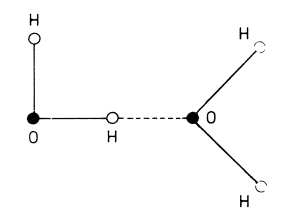
\includegraphics[width=0.6\textwidth]{img/grafico5.17.png}
    \caption{\label{fig:grafico_5_17} Fig. 5.17. [Tres relaciones diferentes entre dos moléculas de agua. (a) Los enlaces de valencia
    entre los componentes atómicos de cada molécula (líneas continuas); (b) el enlace de hidrógeno
    entre ambas moléculas (línea punteada); (c) la relación de estar a la izquierda (o su inverso).
    Tanto (a) como (b) son enlaces, vínculos o acoplamientos, mientras que (c) es una relación sin enlace. ].}
    \end{figure}

    La colección de vínculos entre los miembros de un conjunto arbitrario T de
    cosas merece un nombre especial:

    DEFINICIÓN 5.33 El vínculo de un conjunto T de cosas es el conjunto IBT de todos los
    vínculos entre los miembros de T.

    \bigskip

    \begin{center}
        CAPÍTULO 5
    \end{center}

    
    En principio, la IBT incluye enlaces de todas las n-aridades: diádicos, triádicos, etc.
    En la práctica, los enlaces diádicos o binarios son, con mucho, los más
    importantes. Si solo se tienen en cuenta los enlaces binarios, la definición anterior
    se reduce a

    \begin{center}
        \[
        \begin{gathered}
        \mathbb{B}_{T} = \{ B_{i} \in \text{Binary relations on T} \mid (\exists x)(\exists y) \\
        (x, y \in T \ \& \ B_{i}xy \ \& \ 1 \le i \le m) \},
        \end{gathered}
        \]
    \end{center}

    donde m ~ 1 es el número de tipos de vínculos binarios [o de acción] que existen
    entre los miembros de T.
    Recordemos que hemos supuesto que hay un número finito de propiedades sustanciales generales
    (Postulado 2.3). Por lo tanto, tenemos

    COROLARIO 5.13 El número de vínculos de cualquier conjunto de cosas es finito.
    La clase de todas las relaciones no vinculantes (o «meras») entre Ts se
    designará por BT. Y la unión de IBT y BT es, por supuesto, igual al conjunto de
    todas las relaciones en T. Este concepto será crucial en nuestro tratamiento del
    concepto de sistema concreto en el vol. 4, cap. 7, por lo que invita a la
    
    DEFINICIÓN 5.34 Sea T un conjunto de cosas y [T] su agregación
    [suma física]. Entonces, la estructura de [T] es igual a la totalidad de las relaciones,
    tanto vinculantes como no vinculantes, en T:

    \begin{center}
        \[ \mathcal{S}([[T]]) = \mathbb{B}_{T} \cup \overline{\mathbb{B}_{T}}. \]
    \end{center}

    Utilizaremos el concepto de enlace para caracterizar los sistemas y los
    marcos de referencia.

    \subsection{Agregados y sistemas}
    Ahora emplearemos los conceptos de enlace e historia para aclarar la
    distinción entre un montón o agregado, por un lado, y un todo
    o sistema, por otro. Ejemplos obvios de sistemas son los átomos y las
    moléculas. Por otro lado, los nucleones y electrones que componen un
    átomo no son sistemas, ya que no tienen componentes separables.
    Otro ejemplo de no sistema es el agregado formado por una cosa y
    un marco de referencia. Dado que se supone que los marcos de referencia registran
    sin influir ni ser influenciados, la historia de un compuesto cosa-marco debe reflejar esa independencia. Cómo se hace esto se
    verá en la sección 4.3, una vez que hayamos introducido adecuadamente la noción de
    sistema.

    \begin{center}
        CAMBIO
    \end{center}

    Un análisis de las historias de los miembros de un conjunto de cosas debería
    ayudarnos a descubrir si la agregación del conjunto constituye o no un
    sistema, es decir, si sus componentes están unidos o no. De hecho, la
    historia de un agregado de cosas que no interactúan entre sí está determinada de forma única
    por las historias de dichos componentes: es simplemente su unión. No es así en el
    caso de un sistema: aquí la historia de cada componente está determinada, al
    menos en parte, por los estados en los que se encuentran los demás componentes, de modo que la historia del
    conjunto no es igual a la suma de las historias individuales. Uno
    o dos ejemplos ayudarán a entender este punto.

    Piensa en las historias de una polilla y una vela antes y después de que
    la primera se precipite en espiral hacia la segunda. Si se necesita un ejemplo más distinguido,
    piensa en un sistema compuesto por dos electrones lo suficientemente cercanos como para interactuar
    de forma apreciable, como es el caso de los de un átomo de helio. Este sistema se
    describe mediante una ecuación de Schrodinger (clásicamente mediante dos ecuaciones de movimiento acopladas) junto con el principio de exclusión de Pauli. Este último
    selecciona aquellas funciones de estado que son impares (antisimétricas) en las coordenadas de los electrones. (Es decir, la ley adicional es: $: \psi(x, y) = -\psi(y, x),$,
    donde x e y son las coordenadas de posición de los electrones. De ello se deduce
    que $\psi(x, x) = \dot{0}$, es decir, las dos entidades no pueden coexistir en el mismo punto,
    a menos que tengan espines diferentes). El principio de Pauli expresa una propiedad global
    o sistémica, que los componentes individuales no poseen,
    por lo que no puede representarse en los espacios de estado parciales. Por lo tanto,
    la construcción del espacio de estado del sistema debe partir de
    cero, en lugar de basarse únicamente en los espacios de estado de los electrones individuales.
    (Afortunadamente, el principio de Pauli no se aplica a todo el
    universo, sino solo a ciertas partes del mismo, concretamente a los subsistemas formados
    por componentes de espín medio entero. De lo contrario, no existirían sistemas bastante
    aislados en la realidad. (0. Margenau (1966).)) Lo que se aplica a los espacios de estado
    se aplica con mayor razón a las historias.
    Resumimos y generalizamos las observaciones anteriores en

    DEFINICIÓN 5.35 Sea X una cosa compuesta de partes para $X_{i} \ \text{for} \ 1 \le i \le n$.
    Entonces X es un agregado (o conglomerado o montón) si y solo si, en cada representación de X (es decir, para cada elección de función de estado), su historia h(X)
    es igual a la unión de las historias parciales h(~). De lo contrario, X es un sistema.
    La cautelosa frase «en cada representación», que aparece en la convención anterior, se debe a esto. A menudo es posible elegir una
    representación de una cosa en la que las acciones mutuas de sus componentes
    se «absorben» en esta última. En otras palabras, a menudo se puede modelar lo real

    \begin{center}
        CAPÍTULO 5
    \end{center}

    sistema como un agregado conceptual de componentes que no interactúan entre sí. Pero
    este truco no funciona para todas las representaciones.
    Recordando las definiciones 5.31 de acción y 5.33 de servidumbre, obtenemos el

    COROLARIO 5.14 Sea X una cosa con composición <€(X). Entonces X es un
    sistema si y solo si la unión de <€(X) no está vacía, es decir, B~(X) ¢ 0.

    Ahora bien, el universo o mundo es aquella cosa que está compuesta por todas las
    cosas (Postulado 3.3); y según el Postulado 5.10, cada cosa —por lo tanto, cada
    componente del mundo— está unida a alguna otra cosa. Por lo tanto, 

    COROLARIO 5.15 El mundo o universo es un sistema.
    Por la Definición 5.35 se deduce a su vez que la historia del mundo no es
    igual a la unión de las historias de sus partes.

    ¿Qué ocurre si un sistema se desintegra, por ejemplo, si sus componentes se separan
    y dejan de interactuar? Parecería que, cuando esto ocurre, la historia
    del conjunto es igual a la unión de las historias de los antiguos
    componentes, que ahora están libres unos de otros. Esto no es necesariamente así. De hecho, la famosa paradoja de Einstein-Podolsky-Rosen de la mecánica cuántica puede interpretarse de la siguiente manera. Si dos cosas cuánticas
    interactúan en un momento dado, incluso después de haber dejado de interactuar,
    siguen estando correlacionadas en el sentido de que la historia de cada una se ve afectada por
    lo que le sucede a la otra. (De manera equivalente: el vector de estado del todo
    no es igual al producto directo de los vectores de estado de las partes). Por lo tanto,
    la interacción en algún momento es suficiente para inducir una correlación que se
    refleja en la indivisibilidad del espacio de estado total y, a
    mayor razón, en la inseparabilidad de las historias parciales. Si esta interpretación es correcta, entonces se pueden mantener las definiciones anteriores, pero se debe añadir una nueva
    suposición: una vez que es un (micro)sistema, siempre es un (micro)sistema. Sin embargo, esto sigue siendo discutible, por lo que no lo incorporaremos al
    sistema solar.

    \subsection*{4.3 Marco de referencia}


    Otra aplicación importante del concepto de agregado es la caracterización de un marco de referencia. Este concepto es de suma
    importancia no solo en física, sino también en nuestra ontología, ya que en casos reales
    los estados dependen del marco. (El paradigma es, por supuesto, el estado de
    movimiento de un cuerpo: su trayectoria en el espacio de estados depende del marco. Tanto es así
    que no se moverá en absoluto en relación con un marco rígidamente unido a sí mismo). 

    \bigskip

    \begin{center}
        CAMBIO
    \end{center}

    Una condición para que una cosa pueda servir de marco de referencia para otra es
    que ambas no se influyan mutuamente, de modo que sus respectivos estados estén
    claramente separados. (Para caer en el antropomorfismo: un marco de referencia
    debe ser un espectador imparcial. Pero esto es solo un recurso didáctico: no debemos
    confundir los marcos con los observadores). Otra condición es que los estados
    del marco de referencia de una cosa determinada sean utilizables para parametrizar
    los estados de la cosa de interés, en el sentido de que, para cada estado t del
    marco de referencia, la cosa se encuentre en un estado determinado s = 1F(t), donde IF es la
    función de estado de n componentes para la cosa. (Véase la figura 5.18) Estas dos 

    \begin{center}
        \begin{figure}[h!]
        \centering
        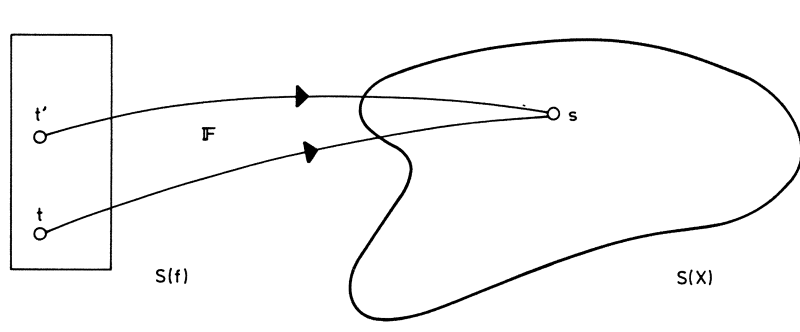
\includegraphics[width=0.6\textwidth]{img/grafico5.18.png}
        \caption{\label{fig:grafico_5_18} Fig. 5.18. [La correspondencia IF: S(j)-'> S(X) de estados de referencia a estados de cosas. IF no tiene por qué
        ser 1-1: dos estados de referencia diferentes pueden corresponder a un único estado de cosa, como en el
        movimiento periódico. Pero IF debe ser sobre: cada estado de cosa debe emparejarse con al menos un
        estado de referencia. ].}
        \end{figure}
    \end{center}
    Las condiciones —independencia y parametrizabilidad— se considerarán
    conjuntamente necesarias y suficientes para caracterizar el concepto general de un
    marco de referencia. (Cada teoría científica puede definir su propio concepto específico
    de marco de referencia añadiendo sus propias condiciones adicionales,
    normalmente que se cumplan ciertas leyes en relación con el marco. Véase Bunge
    (1967b). En resumen, hacemos la
    DEFINICIÓN 5.36 Sea X una cosa representada por el esquema funcional
    Xm = (M, IF) y sea f otra cosa con estados en S(f). Entonces f
    es un marco de referencia para X si y solo si
    (i) f + X es un agregado, de modo que h(f + X) = h(f) u h(X), y
    (ii) el dominio de la función de estado de X es igual al espacio de estados de f,
    es decir, IF: S(f) ~ S(X), de donde M = S(f)).

  \bigskip

  Observación 1 Hemos definido un marco de referencia como algo concreto de un
  cierto tipo. Dado que cada marco de referencia puede representarse mediante un
  parche de coordenadas en una variedad, se ha extendido la idea errónea de que
  los marcos de referencia son idénticos a sus representantes conceptuales.
  Que esto es un error se comprende al recordar que a los marcos se les asignan
  propiedades sustanciales, como velocidades, lo que sería imposible si
  fueran conceptos. Observación 2: un marco de referencia no tiene por qué ser un
  cuerpo perfectamente rígido. Esto es así, en primer lugar, porque no existe tal cosa como un
  cuerpo rígido en el mundo real y, en segundo lugar, porque un marco debe tener
  partes móviles para poder funcionar como un reloj (natural o artificial). Un
  marco puede ser un campo (Dehnen, 1970).
  El concepto de marco de referencia nos permite dilucidar la noción de que una
  cosa se encuentra en un estado determinado en relación con algún marco. De hecho, podemos
  introducir

      \bigskip
      
    \noindent\textbf{DEFINICIÓN 5.37} Sea $f$ un marco de referencia para una cosa $X$ representada por el esquema funcional $X_m = (S(f), F)$. Entonces
    \begin{enumerate}
        \item[(i)] el \textbf{estado} de $X$ en $t \in S(f)$ relativo a $f$ es
        $$ s = F(t) = \langle F_i(t) | 1 \le i \le n \rangle; $$

        \item[(ii)] el \textbf{espacio de estados} de $X$ relativo a $f$ es
        $$ S(X) = \{s = F(t) | t \in S(f)\} = F(S(f)). $$
    \end{enumerate}
  \bigskip
  Debido a que existe un número ilimitado de marcos de referencia, y la
  elección del esquema funcional para representar una cosa es en parte convencional,

  los estados pueden parametrizarse de varias maneras. Algunas de estas representaciones
  son equivalentes, como cuando los marcos son inerciales en cierto sentido,

  mientras que otras no lo son. Esto no implica que los estados sean realmente absolutos
  (independientes del marco) y que debamos culpar a nuestras propias limitaciones cognitivas
  por la relatividad de los estados. Excepto en el caso altamente artificial
  en el que se supone que todos los componentes de una función de estado son invariables
  bajo todas las posibles sustituciones de marcos, los estados en sí mismos son relativos.
  Esto es suficiente para considerar con recelo todas las teorías filosóficas
  que emplean descripciones absolutas de los estados, como «La cosa X está en el estado s»
  o, peor aún, «El estado del mundo en un instante dado es tal y tal».
  (La metafísica de los mundos posibles y la lógica inductiva abundan en tales
  curiosidades). Pero la relatividad no debe confundirse con la subjetividad: que
  cada estado de una cbosa sea relativo a un marco no implica que sea el
  estado privado de un sujeto, a menos que, por supuesto, se confunda la cosa

  
      \noindent
      estados con estados de referencia o estados de un estándar de referencia, y
  marcos con sujetos u observadores. (Para críticas sobre tales confusiones, véase
  Bunge, 1967b, 1973b).

  Hasta aquí los tecnicismos. Pasemos ahora a algunas cuestiones de principio bastante menos técnicas,
  pero igualmente importantes.
  \bigskip
  \section{\centering PANTA RHEI}
    \subsection{Hecho}
    
  Ahora que disponemos de definiciones exactas de estado (cap. 3, sec. 2) y de
  cambio de estado o acontecimiento (sec. 2), podemos comprender plenamente la definición
  4.3 de hecho. Ahora podemos decir que un hecho (real) es o bien la existencia de una cosa
  en un estado determinado, o bien un acontecimiento que ocurre en una cosa. Se me ocurren los siguientes comentarios
  .
  En primer lugar, la definición anterior de un hecho se aplica también al caso de la
  conversión de una cosa (por ejemplo, una oruga) en otra (por ejemplo, una mariposa),
  siempre que interpretemos ambas cosas como una sola cosa en dos etapas sucesivas
  de desarrollo. De hecho, como se sugiere en la sección 1.2, todo lo que tenemos que hacer
  es fingir que estamos tratando con una misma cosa cuyo
  punto representativo se mueve ahora en un espacio de estado (por ejemplo, el espacio de estado de la oruga),
  ahora en otro (por ejemplo, el espacio de estado de la mariposa), estando los dos espacios de estado
  correctamente ensamblados.
  En segundo lugar, las construcciones —como los conceptos y las proposiciones— no
  se consideran hechos, ya que no son ni estados de las cosas ni cambios en
  las cosas. Por lo tanto, es erróneo llamar hecho a una proposición factual verdadera. A
  penas, una proposición podría considerarse como una cierta clase de equivalencia de
  estados mentales, pero una clase es un concepto, no una cosa. Por lo tanto, es erróneo
  identificar ambos.
  En tercer lugar, nuestra interpretación de los hechos es objetiva. No definimos un hecho como
  «cualquier cosa que pueda observarse» porque (a) la microfísica,
  la megafísica y la fisiología de la percepción nos enseñan que la mayoría de los hechos

  permanecen más allá de la observación humana (aunque nofue el caso de Russell (1914), Whitehead (1919), Carnap (1928)

  y Goodman (1951), uno se abstendrá de definir conceptos ontológicos
  en términos semánticos, epistemológicos o psicológicos; (b) la mayoría de

  las proposiciones fácticas son, en el mejor de los casos, parcialmente verdaderas en lugar de totalmente verdaderas; (c)
  la definición semántica de un hecho obliga a afirmar que existen
  hechos negativos (los que verifican afirmaciones negativas) y hechos generales

  (los que confirman afirmaciones generales). La extraña metafísica de los hechos negativos
  y generales se evita si, contrariamente al Wittgenstein temprano

  y al Russell del atomismo lógico, se abandona la suposición de que

  las proposiciones y los hechos tienen una correspondencia 1-1. La correspondencia
  no puede ser tal porque todos los hechos son «positivos» y singulares.

  (Recordemos que un hecho es o bien el ser de una cosa en un estado, o bien la
  ocurrencia de un cambio de estado de una cosa). La no ocupación de un estado
  y la no ocurrencia de un evento no son hechos. Por lo tanto, no haber sido
  vacunado contra la viruela no es un evento, por lo que no cuenta como una
  causa de la viruela. Y como no admitimos eventos negativos,
  evitamos hablar de «eventos lógicos» como «e o no e», por lo que no
  tenemos que preocuparnos por sus causas. Consideramos que esto es una ventaja distintiva
  sobre la teoría probabilística de la causalidad (Suppes, 1970),
  en la que cualquier elemento de un espacio de probabilidad se considera un evento y en la que
  se supone que la relación causal se da entre eventos posibles, incluso
  los negativos, en lugar de entre eventos reales. En resumen, es falso que
  todo lo que hace que una proposición sea verdadera o falsa cuente como un hecho.

  En quinto y último lugar, los hechos, ya sean posibles o reales, son objetivos, pero,
  según Wittgenstein (1922), no constituyen el mundo. El mundo

  no es la totalidad de los hechos, sino la totalidad de las cosas, es decir, individuos concretos
  dotados de todas sus propiedades, algunas de las cuales consisten en
  su capacidad de cambiar de manera definida (aunque posiblemente aleatoria) y legal
  . Así es como tanto la cosmología física como nuestra ontología interpretan
  el término «mundo». La interpretación de Wittgenstein requiere o bien prescindir

  por completo de las cosas —una situación incómoda para la ciencia— o bien intentar
  definirlas en términos de hechos, intento que ni siquiera se ha

  abordado. Más sobre esto en la sección 6.

      \noindent 
  \bigskip
  \subsection{Dinamismo}

  El nuestro es un mundo de cosas, pero de cosas cambiantes, no estáticas.
  De hecho, según el postulado ~U 1 de la sección 4.1, cada cosa tiene una
  historia no trivial. En otras palabras, cada cosa cambia. Esta es nuestra versión

  CAMBIO 269
  del panta rhei de Heráclito. Tenga en cuenta que aún no estamos tomando una postura
  con respecto a la hipótesis ontológica más fuerte de que todas las cosas cambian
  incesantemente: aún no tenemos un concepto adecuado del tiempo. Para que el Postulado
  5.11 sea válido, es necesario y suficiente que todas las cosas cambien al menos
  una vez, es decir, que la historia de todas las cosas consista en al menos dos estados o,
  equivalentemente, en un evento.
  Damos por sentado el cambio —no su concepto— en lugar de negarlo
  o justificarlo. Lo que hay que justificar en cada caso no es el cambio, sino
  cualquier suposición o pretensión de que una determinada cosa no
  cambia en algún aspecto. Hacemos este tipo de cosas todo el tiempo, al decir
  que ciertos cambios, aunque reales, son pequeños, o que no consisten en
  nada más que en movimiento relativo, etc. Además, explicamos la permanencia (en
  ciertos aspectos) en términos de aislamiento, o equilibrio de
  fuerzas, o lo que sea. La estática es un caso particular de la dinámica, la electrostática
  de la electrodinámica, y así sucesivamente. Las teorías más poderosas y profundas de la
  ciencia contemporánea son teorías del cambio, no teorías del ser:
  la permanencia es un caso particular, excepcional y temporal de cambio. Negar
  que todas las cosas están en constante movimiento, negar que el cambio universal es
  objetivo —como han hecho Weyl (1949), Costa de Beauregard (1963) y Griinbaum
  (1967), es un ejercicio de sofistería.
  La visión dinamista inherente a la ciencia contemporánea, y adoptada
  por nuestra ontología, contrasta no solo con el estaticismo parmenideo, sino también
  con la hipótesis aristotélica y tomista de que el reposo, y no
  el movimiento, es el estado «natural» de las cosas. Nuestra versión del dinamismo va
  un paso más allá de la de Demócrito, para quien los átomos en sí mismos
  no estaban sujetos a cambios. Tanto la física de alta como la de baja energía sugieren que ni
  siquiera los componentes «últimos» de las cosas —las «partículas elementales» y

  los campos— están en reposo. No existe la materia inerte, ni la materia perpetuamente inmutable
  que solo puede ser perturbada por influencias externas, pero que

  por lo demás es pasiva. Como vio Bolzano, tales influencias externas y los
  movimientos relativos resultantes no podrían explicarse «si no pudiera
  producirse ningún cambio en el interior de las sustancias simples mismas»; por lo tanto,
  «la capacidad de cambio a través de la influencia mutua» debe atribuirse
  a todas las sustancias, ya sean complejas o simples (Bolzano, 1851, §§ 50, 51).
  El «polo inmutable» exaltado por algunos poetas y filósofos no es una
  cosa o un conjunto de cosas, sino el conjunto de leyes objetivas básicas.
  Nuestra visión es definitivamente dinamista, pero no en exceso; asumimos
  que todo cambia en algún aspecto u otro, pero nos abstenemos de
  afirmar que cambia en todos los aspectos, y mucho menos de forma incesante. Ciencia
    \noindent

    \bigskip
    no parece respaldar tal exageración: muestra que algunos rasgos
  permanecen invariables a lo largo de ciertos cambios. (Las constantes del
  movimiento de un sistema físico se encuentran entre tales invariantes). Además,
  el cambio en algunos aspectos solo es posible gracias a la permanencia en

  otros. (Por lo tanto, los procesos vitales son imposibles a menos que se mantenga la homeostasis).
  Del mismo modo, todo lo que es permanente (invariante, inmutable) lo es

  en relación con (bajo) un conjunto específico (grupoide, semigrupo o grupo) de
  transformaciones. En consecuencia, las invariantes de cualquier estructura de este tipo
  pueden no ser las mismas que las de un conjunto diferente de transformaciones.
  Lo que se aplica a cada cosa individual —es decir, que es cambiante— es
  cierto para la cosa compuesta de todas las cosas, es decir, el universo. Es decir, el
  mundo en su conjunto está en constante cambio, aunque no como un único sistema
  o cosmos bien integrado. El flujo universal es un enorme conjunto de procesos, algunos de los
  cuales se entrelazan (se influyen mutuamente), mientras que la mayoría probablemente no lo hacen.
  Por lo tanto, es erróneo hablar de «la serie mundial de acontecimientos», como si
  se tratara de algo parecido a una serie mundial de béisbol a gran escala. A fortiori, es
  erróneo afirmar o negar que dicha serie tenga un principio o un fin.
  Simplemente no existe una serie mundial de acontecimientos. Dado que la relación de precedencia
  entre los acontecimientos es local (vinculada a un marco de referencia u otro), la
  totalidad de los acontecimientos no tiene un orden general. Todo lo que podemos afirmar —y de hecho hemos
  afirmado en el Postulado 5.9— es que cada proceso individual está precedido
  y seguido por otros procesos. Por lo tanto, aunque el mundo en su conjunto
  no participa en una carrera de relevos, cada parte de él participa en alguna
  carrera de relevos local u otra.
      \noindent
      \bigskip
      \subsection{Interconexión}
      El postulado 5.10 de la sección 4.1 establece que todo influye o es
  influenciado por otras cosas. En otras palabras, nada, excepto
  el universo en su conjunto, está totalmente aislado. Si esto es así, entonces el mundo es
  un todo interconectado, es decir, un sistema más que un agregado. (Recuerde
  la definición 3.12 del capítulo 3, sección 2.7). Sin embargo, no es un todo muy cohesionado.

  La hipótesis de que el mundo es un sistema es más débil, pero presumiblemente
  más cercana a la verdad, que la cosmología organicista de Platón, los estoicos o
  Hegel, según los cuales cada cosa está unida a todas las demás, de modo que
  el mundo en su conjunto es un «todo orgánico». Si esta otra hipótesis
  fuera cierta, sería imposible estudiar cualquier cosa en particular
  sin tener en cuenta todas las demás, y sería imposiblemente
  capaz de actuar sobre cualquier cosa en particular sin perturbar todo el
  universo.
  Tanto la ciencia contemporánea como nuestra ontología siguen un camino intermedio

  entre los extremos del organicismo («Todo está unido formando un bloque sólido»)
  y el atomismo («Todo va por su propio camino»). Ninguna

  parte del universo está aislada (o completamente libre de vínculos), pero todo
  está aislado en algunos aspectos de otras cosas. Esta interconexión parcial
  de las partes del mundo hace posible su estudio,
  ya que el estudio de cada cosa es parcial y se basa en la posibilidad de
  entrar en contacto con ella.
  Además, el Postulado 5.10 proporciona el criterio de existencia comúnmente
  utilizado en las ciencias, a saber: todo lo que existe (real y físicamente) está
  influenciado por otras cosas o influye en ellas. Repito:
      \noindent
  \bigskip
    CRITERIO 5.1 Para cualquier objeto x distinto del mundo, x existe realmente si y solo si
  hay una cosa y distinta de x tal que y actúa sobre x o x actúa sobre y.
  Si la cosa y que actúa sobre la cosa putativa x o sobre la que actúa esta última es
  controlable por un observador, entonces x es objeto de investigación experimental.
  Pero tal posibilidad de control efectivo es suficiente, no
  necesaria, para conjeturar la existencia.
  En resumen, nuestra ontología incluye la tesis de la interconexión limitada o parcial
  de todas las partes del universo.
    \noindent
    \bigskip
    \subsection{Tres conceptos erróneos}
    
  Hemos definido el cambio con referencia a objetos o cosas concretas.
  Toda colección de acontecimientos es un conjunto de cambios en una cosa u otra. No
  encontramos ninguna utilidad a la ficción de que hay cambios que no
  consisten en modificaciones de los estados de una cosa u otra. Cualquiera que
  afirme que existen tales cambios en la realidad debería presentar pruebas empíricas
  al respecto y proceder a construir una teoría de tales cambios sin cosa (o
  inmateriales).
  Sin embargo, de vez en cuando se encuentra a filósofos e incluso científicos
  que afirman que existen tales cambios sin objeto. Examinemos
  brevemente las afirmaciones sobre tres de estos elementos. Uno de ellos es el proceso de la información,
  que a veces se considera que no se basa en el transporte de
  materia o la propagación de campos. La razón de este concepto erróneo es
  que la teoría estadística de la información es una caja negra o una teoría fenomenológica
  tan general que ignora el tipo preciso de señal que transporta la
  información, el mecanismo de transmisión de la información y el tipo o tipos
  y la cantidad de energía involucrados. Por esta razón, la teoría de la información es una
  teoría no física: es más bien una teoría que puede calificarse como una pieza de
  metafísica científica, ya que trata de una manera extremadamente general un
  género de cosas concretas. Pero, por supuesto, la información es una propiedad de
  ciertos procesos físicos (o químicos o biológicos), a saber, las señales,
  que son procesos de un tipo. Sin señal, no hay transmisión de información.
  Y las señales, repitámoslo, son cadenas de acontecimientos que se producen en cosas concretas
  : la transmisión de información consiste en acontecimientos que se propagan
  a través del espacio y transportan energía. Si se eliminan esos procesos reales, solo
  quedan anécdotas parapsicológicas.
  Otro supuesto ejemplo de cambio no físico pero real es la
  tesis paralelista de que los acontecimientos psíquicos o mentales («conductuales») no
  deben concebirse como cambios en el sistema nervioso del animal
  en cuestión. Si se trata de una cuestión metodológica, puede que fuera válida en
  los inicios de la psicología experimental. Pero ahora se ha vuelto
  desagradable porque bloquea la investigación en psicología fisiológica, y es
  absurdo cuando se toma metafísicamente, es decir, como una reafirmación del dogma gastado
  de que el alma está por encima de la materia. No hay ninguna prueba de que
  exista la ideación sin cerebro, mientras que, por otro lado, hay pruebas definitivas
  de que todo evento mental es un evento en el cerebro de algún animal. Dejamos
  la investigación detallada de este asunto para el vol. 4, cap. 10.
  Un tercer punto de incidencia del inmaterialismo es la teoría cuántica
  mecánica estándar de la medición (von Neumann, 1932). Según
  ella, la diferencia más llamativa entre la física cuántica y la física clásica
  es que, mientras que esta última trata los procesos de medición como procesos puramente
  físicos, según la mecánica cuántica no lo son
  debido a la intervención de la mente del observador y sus decisiones. Tanto es así, se alega, que solo los procesos naturales obedecen a la ecuación de Schrödinger

  (pero entonces son inobservables), mientras que los procesos de medición
  obedecen a una teoría separada centrada en un postulado diferente, a saber,

  el postulado de proyección. Esta interpretación no es aceptada por los
  seguidores ortodoxos de Bohr, según los cuales todos los eventos cuánticos

  (que ellos llaman «fenómenos»), y no solo los controlados por dispositivos de medición,
  implican actos de observación. Según esta visión alternativa,

  no habría microeventos espontáneos (no provocados y no observados)
  («fenómenos cuánticos»). Los realistas rechazan, por supuesto, la tesis de Bohr,
  así como la de von Neumann (Bunge, 1973b). Un argumento a favor de la
  posición realista es que, si bien es cierto que todo proceso de medición es
    \noindent
  \bigskip
  diseñado, ejecutado e interpretado por alguna persona (eventualmente con la
  ayuda de dispositivos automáticos), es un proceso estrictamente físico en lo que respecta a
  lo medido y a lo que mide. Tanto es así que (a)
  algunos procesos de medición pueden automatizarse por completo y (b)

  ninguna de las teorías de medición existentes incluye variables mentales.
  Pero incluso si se tuviera que considerar el sistema más amplio, incluyendo al observador y su personal,

  esto no convertiría la medición en un proceso no físico,
  a menos que, por supuesto, la mente se interpretara como una sustancia inmaterial
  al estilo de Aristóteles y del público (no del secreto)
  Descartes. Pero la física moderna no necesita aliarse con una metafísica obsoleta
  .
  \noindent
  \vspace{0.3cm}
  \section{\centering OBSERVACIONES FINALES}
    \bigskip
    Una polaridad básica en la metafísica tradicional es la del ser y el devenir:
  el acontecimiento se opone a la cosa, el proceso a la materia, el cambio a la estructura. Esta

  oposición no tiene sentido en nuestro sistema, donde cada cambio es la
  transformación de una cosa u otra, y cada cosa está en constante cambio. Esta
  visión, incompatible con gran parte de la metafísica tradicional, es coherente
  con la ciencia: esta última no proporciona ninguna base para plantear la hipótesis de la
  existencia de acontecimientos sin cosas, del mismo modo que no sugiere que pueda
  haber cosas inmutables. Es cierto que las fórmulas de la ciencia teórica no
  siempre contienen variables de cosas de forma explícita, pero el contexto —lo que
  a veces se denomina «la prosa que identifica las variables»— suele
  dejar claro que las fórmulas se refieren a cosas de algún tipo.
  La descripción precisa de cada acontecimiento requiere mencionar la cosa o
  cosas sujetas al cambio en cuestión. Por eso, cualquier axiomatización correcta
  de una teoría científica comienza por hacer suposiciones
  sobre los tipos de cosas a las que se refiere la teoría y termina por
  caracterizar los acontecimientos como cambios en algunas de las propiedades de tales
  referentes. (Véase, por ejemplo, Bunge, 1967b, 1973b). El camino inverso, es decir,
  el de comenzar con los acontecimientos y terminar definiendo las cosas, ha sido
  sugerido como programa (por ejemplo, por Russell (1914) y Whitehead (1929)),
  pero nunca se ha llevado a cabo. Echemos un vistazo a ello.
  Algunos filósofos del proceso, ansiosos por seguir insistiendo en la
  ontología parmenidea —han llegado al extremo de postular que el
  ser de una entidad consiste en su devenir, que «el mundo real es un
  proceso» (Whitehead, 1929, pp. 29 y passim). Del mismo modo, el físico
  Fokker caracterizó la realidad como una corriente de acontecimientos (Fokker, 1965, p. 1).
  Otros físicos han reinventado esta idea e incluso han negado la
  existencia de las cosas (Bohm, 1970; Finkelstein, 1973; Stapp, 1976). Esta
  idea, de que los acontecimientos y los procesos son la materia de la que está hecho el mundo, ha
  sido fomentada por una terminología engañosa introducida por algunos
  trabajadores de la física relativista, que llaman acontecimiento a cualquier punto del espacio-tiempo,
  independientemente de que ese punto esté ocupado por alguna cosa. Además,
  llaman mundo al conjunto de todos esos «acontecimientos», incluso en el caso de un universo vacío.
  De este modo, el mundo se considera un conjunto de acontecimientos y se pierden de vista las cosas que
  cambian.

  De hecho, no es el mundo, sino solo una línea mundial, un tubo o una historia
  —la región del espacio-tiempo explorada por algo— lo que se considera una secuencia

  de acontecimientos o procesos. (Véase la figura 5.19.) Lo que se puede decir es que cualquier
  región del espacio-tiempo es la sede de posibles eventos que ocurren a las cosas
  (partículas, campos, etc.) que podrían existir dentro de esa región. Pero esto está muy
  lejos de identificar un evento con un cuádruple de números reales.
  En cualquier caso, no necesitamos dedicar más tiempo a la pintoresca versión de la
  metafísica del proceso que prescinde del concepto de cosa, porque es
  lógicamente insostenible. De hecho, es circular definir una cosa como la
    \noindent
  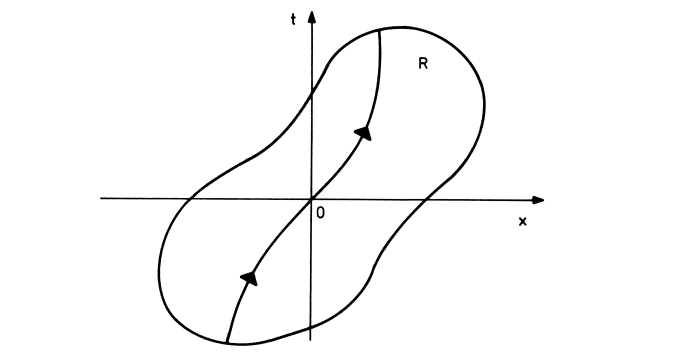
\includegraphics[width=0.9\textwidth]{img/latex2.png}

  Fig. 5.19. La trayectoria espacio-temporal de una partícula puntual (o línea mundial de esta última) es un
  proceso en el espacio-tiempo. A menos que haya realmente otras cosas en la región espacio-temporal
  R, todos los puntos que no constituyan la línea mundial de la partícula son irrelevantes
  y, por lo tanto, no merecen ser llamados «eventos».

  \bigskip
  colección de acontecimientos que ocurren en la cosa. Por eso nuestro estudio del
  cambio fue precedido por un examen del concepto de cosa.
  El dualismo de la metafísica del proceso es, por supuesto, la metafísica del ser. Una

  versión de ello es el estructuralismo, actualmente en boga en Francia (cf. Uvi-
  Strauss, 1958). Al igual que la metafísica tradicional oponía el ser al devenir
  (o la cosa al proceso), e incluso ensalzaba uno de ellos a expensas del

  otro, el estructuralismo tiende a oponer la estructura al cambio y a
  separar la primera de las cosas. Al igual que los dinamistas extremos hablan de
  acontecimientos sin cosas, los estructuralistas hablan de estructuras en sí mismas y
  concentran su atención en la permanencia estructural en medio del flujo. Esto
  también es erróneo: excepto en las matemáticas puras, donde hay estructuras
  en sí mismas —por ejemplo, las álgebras booleanas—, toda estructura es la estructura de

  alguna cosa (compleja): átomo, molécula, célula, órgano, organismo, comunidad,
  ecosistema o lo que sea. (Recordemos la definición 5.34 de la estructura
  de una agregación de cosas). No decimos de un determinado objeto físico

  que es un grupo de rotación, sino que una determinada propiedad del mismo (por ejemplo, la
  energía) tiene simetría de rotación, o es invariante bajo rotaciones (miembros
  del grupo de rotación). Del mismo modo, no decimos de una comunidad que es una
  estructura social, sino que tiene tal estructura. Además, dada
  la mutabilidad de todas las cosas, es poco probable que haya algo con una
  estructura permanente. En resumen, la estructura es una propiedad, y una propiedad
  mutable.

  En conclusión, ni el procesismo ni el estructuralismo son alternativas viables
  a nuestra metafísica de las cosas cambiantes. El devenir no es puro flujo,

  sino que consiste en el ser de las cosas en estados sucesivos, o en cosas sucesivas.
  (Recuerde la Física de Aristóteles, libro III, capítulo 1, sección 1: «no existe tal
  cosa como el movimiento por encima de las cosas»). Y las estructuras no solo son
  volubles, sino que también carecen de existencia independiente: son estructuras de
  las cosas, características de objetos concretos. En resumen, el cambio y la estructura son
  características distintas pero entrelazadas de las cosas cambiantes dotadas de
  alguna estructura u otra. Por lo tanto, los polos metafísicos tradicionales,
  a saber, la metafísica del proceso y la metafísica del ser, tienen cada uno una pizca de
  verdad y ambos son superados por nuestra ontología.
  Llegamos al final de nuestro estudio del cambio en general. Hemos
  formado los principales bloques de construcción para construir los conceptos de tiempo
  y espacio. Una vez que estos estén disponibles, podremos dar una
  explicación más detallada del cambio, en particular del cambio cualitativo,
  que nos ocupará en el vol. 4, cap. 8. Pasamos entonces al estudio de la
  extensión y la duración.

\end{justifying}